%
%   Prof. Dr. Julian Reichwald
%   auf Basis einer Vorlage von Prof. Dr. Jörg Baumgart
%   DHBW Mannheim
%
%
%	ACHTUNG: Für das Erstellen des Literaturverzeichnisses wird das modernere Paket biblatex
%			 in Kombination mit biber verwendet -- nicht mehr das ältere BibTex!
% 			 Bitte stellen Sie ggf. Ihre TeX-Umgebung
% 			 entsprechend ein (z.B. TeXStudio: Einstellungen --> Erzeugen --> Standard Bibliographieprogramm: biber)
%

\documentclass[
	12pt,
	BCOR=5mm,
	DIV=12,
	headinclude=on,
	footinclude=off,
	parskip=half,
	bibliography=totoc,
	listof=entryprefix,
	toc=listof,
	pointlessnumbers,
	plainfootsepline]{scrreprt}

%	Konfigurationsdatei einziehen
% !TEX root =  master.tex

%		LANGUAGE SETTINGS AND FONT ENCODING 
%
\usepackage[ngerman]{babel} 	% German language
\usepackage[utf8]{inputenc}
\usepackage[german=quotes]{csquotes} 	% correct quotes using \enquote{}
\usepackage[T1]{fontenc}
\usepackage{smartdiagram}
\smartdiagramset{border color=black, uniform color list=gray!60 for 4 items, back arrow disabled=true, arrow color=black}
\usepackage{subfigure}
\usepackage[onehalfspacing]{setspace}
\usepackage{listings,xcolor}
\usepackage{svg}
\usepackage{amsmath}
\definecolor{darkblue}{RGB}{061 045 209}
\definecolor{darkgreen}{RGB}{025 130 004}
\definecolor{darkred}{RGB}{090 000 000}
\definecolor{darkorange}{RGB}{255 076 000}

%\usepackage[english]{babel}   % For english language
%\usepackage{csquotes} 	% Richtiges Setzen der Anführungszeichen mit \enquote{}

% 		HYPERREF
%
\usepackage[
	hidelinks=true % keine roten Markierungen bei Links
	%breaklinks=true
]{hyperref}

% Zwei eigene Befehle zum Setzen von Autor und Titel. Ausserdem werden die PDF-Informationen richtig gesetzt.
\newcommand{\TitelDerArbeit}[1]{\def\DerTitelDerArbeit{#1}\hypersetup{pdftitle={#1}}}
\newcommand{\AutorDerArbeit}[1]{\def\DerAutorDerArbeit{#1}\hypersetup{pdfauthor={#1}}}
\newcommand{\Firma}[1]{\def\DerNameDerFirma{#1}}
\newcommand{\Kurs}[1]{\def\DieKursbezeichnung{#1}}


% Correct superscripts 
\usepackage{fnpct}




%		CALCULATIONS
%
\usepackage{calc} % Used for extra space below footsepline



%		BIBLIOGRAPHY SETTINGS
%

% Uncomment the next three lines for author-year-style with footnotes (Chicago)
\usepackage[backend=biber, autocite=footnote, style=authoryear-ibid, dashed=false]{biblatex} 	
%Use Author-Year-Cites with footnotes
\AdaptNoteOpt\footcite\multfootcite   %will add  separators if footcite is called multiple consecutive times 
\AdaptNoteOpt\autocite\multautocite % will add  separators if autocite is called multiple consecutive times

% Uncomment the next line for IEEE-style 
% \usepackage[backend=biber, autocite=inline, style=ieee]{biblatex} 	% Use IEEE-Style (e.g. [1])

% Uncomment the next line for alphabetic style 
% \usepackage[backend=biber, autocite=inline, style=alphabetic]{biblatex} 	% Use alphabetic style (e.g. [TGK12])

% Uncomment the next two lines vor Harvard-Style 
%\usepackage[backend=biber, style=apa]{biblatex} 	
%\DeclareLanguageMapping{german}{german-apa}


\DefineBibliographyStrings{ngerman}{  %Change u.a. to et al. (german only!)
	andothers = {{et\,al\adddot}},
}

%%% Uncomment the following lines to support hard URL breaks in bibliography 
%\apptocmd{\UrlBreaks}{\do\f\do\m}{}{}
%\setcounter{biburllcpenalty}{9000}% Kleinbuchstaben
%\setcounter{biburlucpenalty}{9000}% Großbuchstaben


\setlength{\bibparsep}{\parskip}		%add some space between biblatex entries in the bibliography
\addbibresource{bibliographycitavi.bib}	%Add file bibliography.bib as biblatex resource


%		FOOTNOTES 
%
% Count footnotes over chapters
\usepackage{chngcntr}
\counterwithout{footnote}{chapter}

%	ACRONYMS
%%%
%%% WICHTIG: Installieren Sie das neueste Acronyms-Paket!!!
%%%
\makeatletter
\usepackage[printonlyused]{acronym}
\@ifpackagelater{acronym}{2015/03/20}
  {%
    \renewcommand*{\aclabelfont}[1]{\textbf{\textsf{\acsfont{#1}}}}
  }%
  {%
  }%
\makeatother

%		LISTINGS
\usepackage{listings}	%Format Listings properly
\renewcommand{\lstlistingname}{Quelltext} 
\renewcommand{\lstlistlistingname}{Quelltextverzeichnis}
\lstset{numbers=left,
	numberstyle=\tiny,
	captionpos=b,
	basicstyle=\ttfamily\small}


%		EXTRA PACKAGES
\usepackage{lipsum}    %Blindtext
\usepackage{graphicx} % use various graphics formats
\usepackage[german]{varioref} 	% nicer references \vref
\usepackage{caption}	%better Captions
\usepackage{booktabs} %nicer Tabs
\usepackage{array}
%\newcolumntype{P}[1]{>{\raggedright\arraybackslash}p{#1}}


%		ALGORITHMS
\usepackage{algorithm}
\usepackage{algpseudocode}
\renewcommand{\listalgorithmname}{Algorithmenverzeichnis }
\floatname{algorithm}{Algorithmus}


%		FONT SELECTION: Entweder Latin Modern oder Times / Helvetica
\usepackage{lmodern} %Latin modern font
%\usepackage{mathptmx}  %Helvetica / Times New Roman fonts (2 lines)
%\usepackage[scaled=.92]{helvet} %Helvetica / Times New Roman fonts (2 lines)

%		PAGE HEADER / FOOTER
%	    Warning: There are some redefinitions throughout the master.tex-file!  DON'T CHANGE THESE REDEFINITIONS!
\RequirePackage[automark,headsepline,footsepline]{scrpage2}
\pagestyle{scrheadings}
\renewcommand*{\pnumfont}{\upshape\sffamily}
\renewcommand*{\headfont}{\upshape\sffamily}
\renewcommand*{\footfont}{\upshape\sffamily}
\renewcommand{\chaptermarkformat}{}
\RedeclareSectionCommand[beforeskip=0pt]{chapter}
\clearscrheadfoot

\ifoot[\rule{0pt}{\ht\strutbox+\dp\strutbox}DHBW Mannheim]{\rule{0pt}{\ht\strutbox+\dp\strutbox}DHBW Mannheim}
\ofoot[\rule{0pt}{\ht\strutbox+\dp\strutbox}\pagemark]{\rule{0pt}{\ht\strutbox+\dp\strutbox}\pagemark}

\ohead{\headmark}


\usepackage[T1]{fontenc}
\usepackage{inconsolata}

\usepackage{color}

\definecolor{pblue}{rgb}{0.13,0.13,1}
\definecolor{pgreen}{rgb}{0,0.5,0}
\definecolor{pred}{rgb}{0.9,0,0}
\definecolor{pgrey}{rgb}{0.46,0.45,0.48}

\usepackage{listings}

\lstset{language=Java,
    showspaces=false,
    showtabs=false,
    breaklines=true,
    showstringspaces=false,
    breakatwhitespace=true,
    commentstyle=\color{pgreen},
    keywordstyle=\color{pblue},
    stringstyle=\color{pred},
    basicstyle=\ttfamily,
    moredelim=[il][\textcolor{pgrey}]{$$},
    %    morecomment=[s][\color{yellow}]{@}{\ },
   moredelim=[is][\textcolor{darkorange}]{\%\%}{\%\%},
    basicstyle=\ttfamily\fontsize{10}{12}\selectfont
}

\begin{document}

%% BITTE GEBEN SIE HIER DEN TITEL UND DIE AUTORIN / DEN AUTOR DER ARBEIT AN!
%% DIESE INFORMATIONEN _MÜSSEN_ GESETZT SEIN, UM TITELBLATT, ABSTRACT UND
%% EIGENSTÄNDIGKEITSERKLÄRUNG AUTOMATISCH ANZUPASSEN!
%\TitelDerArbeit{Visualisierung von Daten des Internet of Things mit besonderer Betrachtung der User Experience für den Verbraucher}
\TitelDerArbeit{Intelligent Cinema Suite}
\Firma{SAP SE}
\Kurs{WWI 17 SE B}

\begin{titlepage}
\begin{minipage}{\textwidth}
		\vspace{-2cm}
		\noindent 
\includegraphics[scale=0.28]{img/firmenlogo.jpg} \hfill   
\includegraphics{img/logo.jpg}
\end{minipage}
\vspace{1.5em}
\sffamily
\begin{center}
	\textsf{\large{}Duale Hochschule Baden-W\"urttemberg\\[1.5mm] Mannheim}\\[2em]
	\textsf{\textbf{UMWI/Fallstudie: Prototyp Online-Reservierung Kino-Tickets }}\\[5mm]
	\textsf{\textbf{\Large{}\DerTitelDerArbeit}} \\[1.5cm]
	\textsf{Studiengang Wirtschaftsinformatik\\ Software Engineering}
	
	\vspace{2em}
	%\textsf{\Large{Sperrvermerk}}
\vfill

\begin{minipage}{\textwidth}

\begin{tabbing}
	Wissenschaftlicher Betreuer: \hspace{0.35cm}\=\kill
	Verfasser: 
		\> Dutzi Jonas, MatrNr \\
		\> Keller Sandra, MatrNr \\
		\> Köhler Dennis, MatrNr \\
		\> Sandig Martin, MatrNr \\
		\> Waage Felix, MatrNr \\
		\> Werner Yvonne, MatrNr \\
		\> Westphal Fabio, MatrNr \\
		\> Zahn Milena, MatrNr \\\\
	Firma: \> \DerNameDerFirma  \\[1.5mm]
	Kurs: \> \DieKursbezeichnung \\[1.5mm]
	Dozent: \> Gregor Tielsch \\[1.5mm]
	Abgabe: \> 11. Februar 2019
\end{tabbing}
\end{minipage}

\end{center}

\end{titlepage}

\pagenumbering{roman} % Römische Seitennummerierung
\normalfont

%--------------------------------
% Verzeichnisse - nicht benötige Verzeichnisse bitte auskommentieren / löschen.
%--------------------------------

%   Sperrvermerk
%\input{nondisclosurenotice}

%	Kurzfassung
%\input{abstract}

%	Inhaltsverzeichnis
\tableofcontents

%	Abbildungsverzeichnis
\listoffigures

%	Tabellenverzeichnis
\listoftables

%	Listingsverzeichnis
\lstlistoflistings

% 	Algorithmenverzeichnis
%\listofalgorithms

% 	Abkürzungsverzeichnis (siehe Datei acronyms.tex!)
\clearpage
\chapter*{Abkürzungsverzeichnis}	
\addcontentsline{toc}{chapter}{Abkürzungsverzeichnis}

\begin{acronym}[RDBMS]
	\acro{ICS}{Intelligent Cinema Suite}
	\acro{CRUD}{Create, Read, Update, Delete}
	\acro{POM}{Project Object Model}
	\acro{DI}{Dependency Injection}
	\acro{IoC}{Inversion of Control}
	\acro{ID}{Identifier}
\end{acronym}

\ohead{Acronyms} % Neue Header-Definition

%--------------------------------
% Start des Textteils der Arbeit
%--------------------------------
\clearpage
\ihead{\chaptername~\thechapter} % Neue Header-Definition (inner header)
\ohead{\headmark} % Neue Header-Definition (outer header)
\pagenumbering{arabic}  % Arabische Seitenzahlen

%	Anleitungs-Datei anleitung.tex einziehen. Auf diese Weise sollten Sie versuchen, für jedes einzelne
% Kapitel eine eigene Datei anzulegen und mittels input-Kommando einzuziehen.
% !TEX root =  master.tex
\chapter{Einleitung}

Kurt Tucholsky schrieb bereits vor Hundert Jahren, was auch heute eine Herausforderung der Teamarbeit darstellt: \enquote{Einer hackt Holz, und dreiunddreißig stehen herum – die bilden die Zentrale.} \newline
Diese Seminararbeit begleitet das Projekt zur Erstellung einer Reservierungswebseite für Kinotickets. Dabei wird insbesondere die Vorgehensweise vom Entwurf bis zur Implementierung beschrieben. Es werden Hintergrundinformationen zu verwendeten Technologien und Methoden geliefert. Außerdem werden Einblicke in die Projektplanung und Zusammenarbeit im Team gegbeben. 
Zunächst wird durch die Analyse einer bestehenden Lösung der Status Quo ermittelt und die Anforderungen in einer Soll-Analyse dargelegt. Anschließend werden verschiedene Entwurfsphasen beschrieben und die dazugehörigen Modelle erläutert. Schließlich wird die Umsetzung dessen anhand von Paradigmen und Beispielen beschrieben.
Darüber hinaus wird auf die Herausforderungen und Möglichkeiten einer realtiv großen Gruppe eingegangen. Die Ansätze, wie die Aufgaben bewältigt wurden, werden ebenso geschildert wie die daraus generierten Learnings. 


%% !TEX root =  master.tex
\chapter{Theoretische Grundlagen} 

	(OPTIONAL - vielleicht als Platzfüller)
% !TEX root =  master.tex
\chapter{Projektplanung}
	
	\section[Projektdefinition]{Projektdefinition {\hfill \normalsize Milena Zahn}}
	Das Ziel des Projektes \enquote{\ac{ICS}} ist die Entwicklung eines Prototypen für die Online-Reservierung von Kino-Tickets. Das Projekt wird mit der vorliegenden Seminararbeit dokumentiert. Mit dem Vorlesungsbeginn am 26.11.2018 wird das Projekt gestartet und endet mit der Abschlusspräsentation am 12.02.2019.
	
	\section[Projektbeteiligte]{Projektbeteiligte{\hfill \normalsize Milena Zahn}}
	An diesem Projekt \ac{ICS} arbeiten acht Personen des Kurses WWI 17 SE B der Dualen Hochschule Baden-Württemberg in Mannheim. Im Rahmen der Lehrveranstaltung \enquote{Fallstudie} des Moduls \enquote{Umsetzung der Methoden der Wirtschaftsinformatik} legen folgende Studenten ihre Prüfungsleistung ab:
	\begin{singlespacing}
	\begin{itemize}
		\item Dutzi Jonas, Matrikelnummer: 6681598
		\item Keller Sandra, Matrikelnummer: 6046520 
		\item Köhler Dennis, Matrikelnummer: 8900967 
		\item Sandig Martin, Matrikelnummer: 8857640 
		\item Waage Felix, Matrikelnummer: 3459154 
		\item Werner Yvonne, Matrikelnummer: 8519757 
		\item Westphal Fabio, Matrikelnummer: 6198411  
		\item Zahn Milena, Matrikelnummer: 7488221 
	\end{itemize}
	\end{singlespacing}

	\section[Feasibility Study]{Feasibility Study{\hfill \normalsize Milena Zahn}}
	Bevor das Projekt \ac{ICS} gestartet ist, wurde zuerst eine Feasibility Study, dt. Machbarkeitsstudie, durchgeführt. Es wurde geprüft, ob alle erforderlichen Voraussetzungen für das Projekt vorhanden sind. Die in dem ersten Studienjahr vermittelten programmiertechnischen sowie methodischen Grundlagen werden angewandt. Durch die Lehrveranstaltung \enquote{Systemanalyse und -entwurf} des zweiten Semesters wurden alle notwendigen Kompetenzen zur objektorientierten Analyse und Entwurf erworben. Durch das Modul \enquote{Programmierung und Programmiertechniken} des ersten und zweiten Semesters kann man Erfahrungen in der Programmiersprache Java voraussetzen. Vor dem Projektstart wurden die Rahmenbedingungen, unter denen das Projekt laufen soll, von dem Dozenten gegeben. Des Weiteren wurde innerhalb der Gruppe besprochen, inwiefern das Projekt in der gegeben Zeit umgesetzt werden kann. Der Prozess, dass unterschiedliche Personen sinnvoll zusammenwirken und vielfältige Fähigkeiten genutzt sowie ausgeglichen werden, stellt eine Herausforderung dar. Die Verständigung und Absprachen der in einem cross-funktionalen Team zusammenarbeiten Personen muss reibungslos funktionieren, damit der Informationsaustausch und die Verteilung der Aufgaben sich positiv auf das Projektergebnis auswirken.
	
	Unter Berücksichtigung der Bedingungen dieses Projekts ist vor allem der enge Zeitrahmen auffällig. Das Projektmanagement ist somit neben der Implementierung des Kino-Reservierungstools an sich eine sehr wichtige Aufgabe. Parallel zu diesem Projekt müssen weitere Prüfungsleistungen sowie Vorlesungen von anderen Modulen des dritten Semesters absolviert und demnach mit berücksichtigt werden. Um diese einzuplanen und ein erfolgreiches Projekt abzuschließen, ist eine Projektplanung essentiell. Laut Christoph Wegmann steht \enquote{Planung und Projekterfolg [...] in direktem Zusammenhang}\autocite[][S. 73]{projektmanagement}. Aus diesen Gründen wurde das Projektmanagement von Anfang an von allen Teammitgliedern durchgeführt und beachtet.
	
	\section[Zeitplanung]{Zeitplanung{\hfill \normalsize Milena Zahn}} \label{projektplan}
	\subsection{Projektzeitplan}
	\enquote{Um die Ergebnisse [...] termingerecht zu erreichen, ist eine entsprechend gute Zeitplanung unabdingbar}\autocite[][S. 90]{projektmanagement}.
	In Abbildung \vref{fig:projektablauf} wird der Projektablauf, der zu Beginn des Projektes aufgestellt wurde, dargestellt. Das Projekt beginnt am 26.11.2018 und endet am 12.02.2019. Innerhalb dieser zwölf Wochen sind drei Iterationen vorgesehen. Im Rahmen einer kurzen Präsentation in KW51 2018 und KW4 2019 werden die in der jeweiligen Iteration erarbeiteten Ergebnisse dem Dozenten sowie dem Kurs vorgestellt. Ziel dieser Präsentationen ist es, den aktuellen Projektstatus vorzustellen und Feedback einzuholen. Außerdem dienen diese Präsenzen dazu, Fragen zu stellen und sonstige Hindernisse zu klären. 
	\begin{figure}[H]
		\centering 
		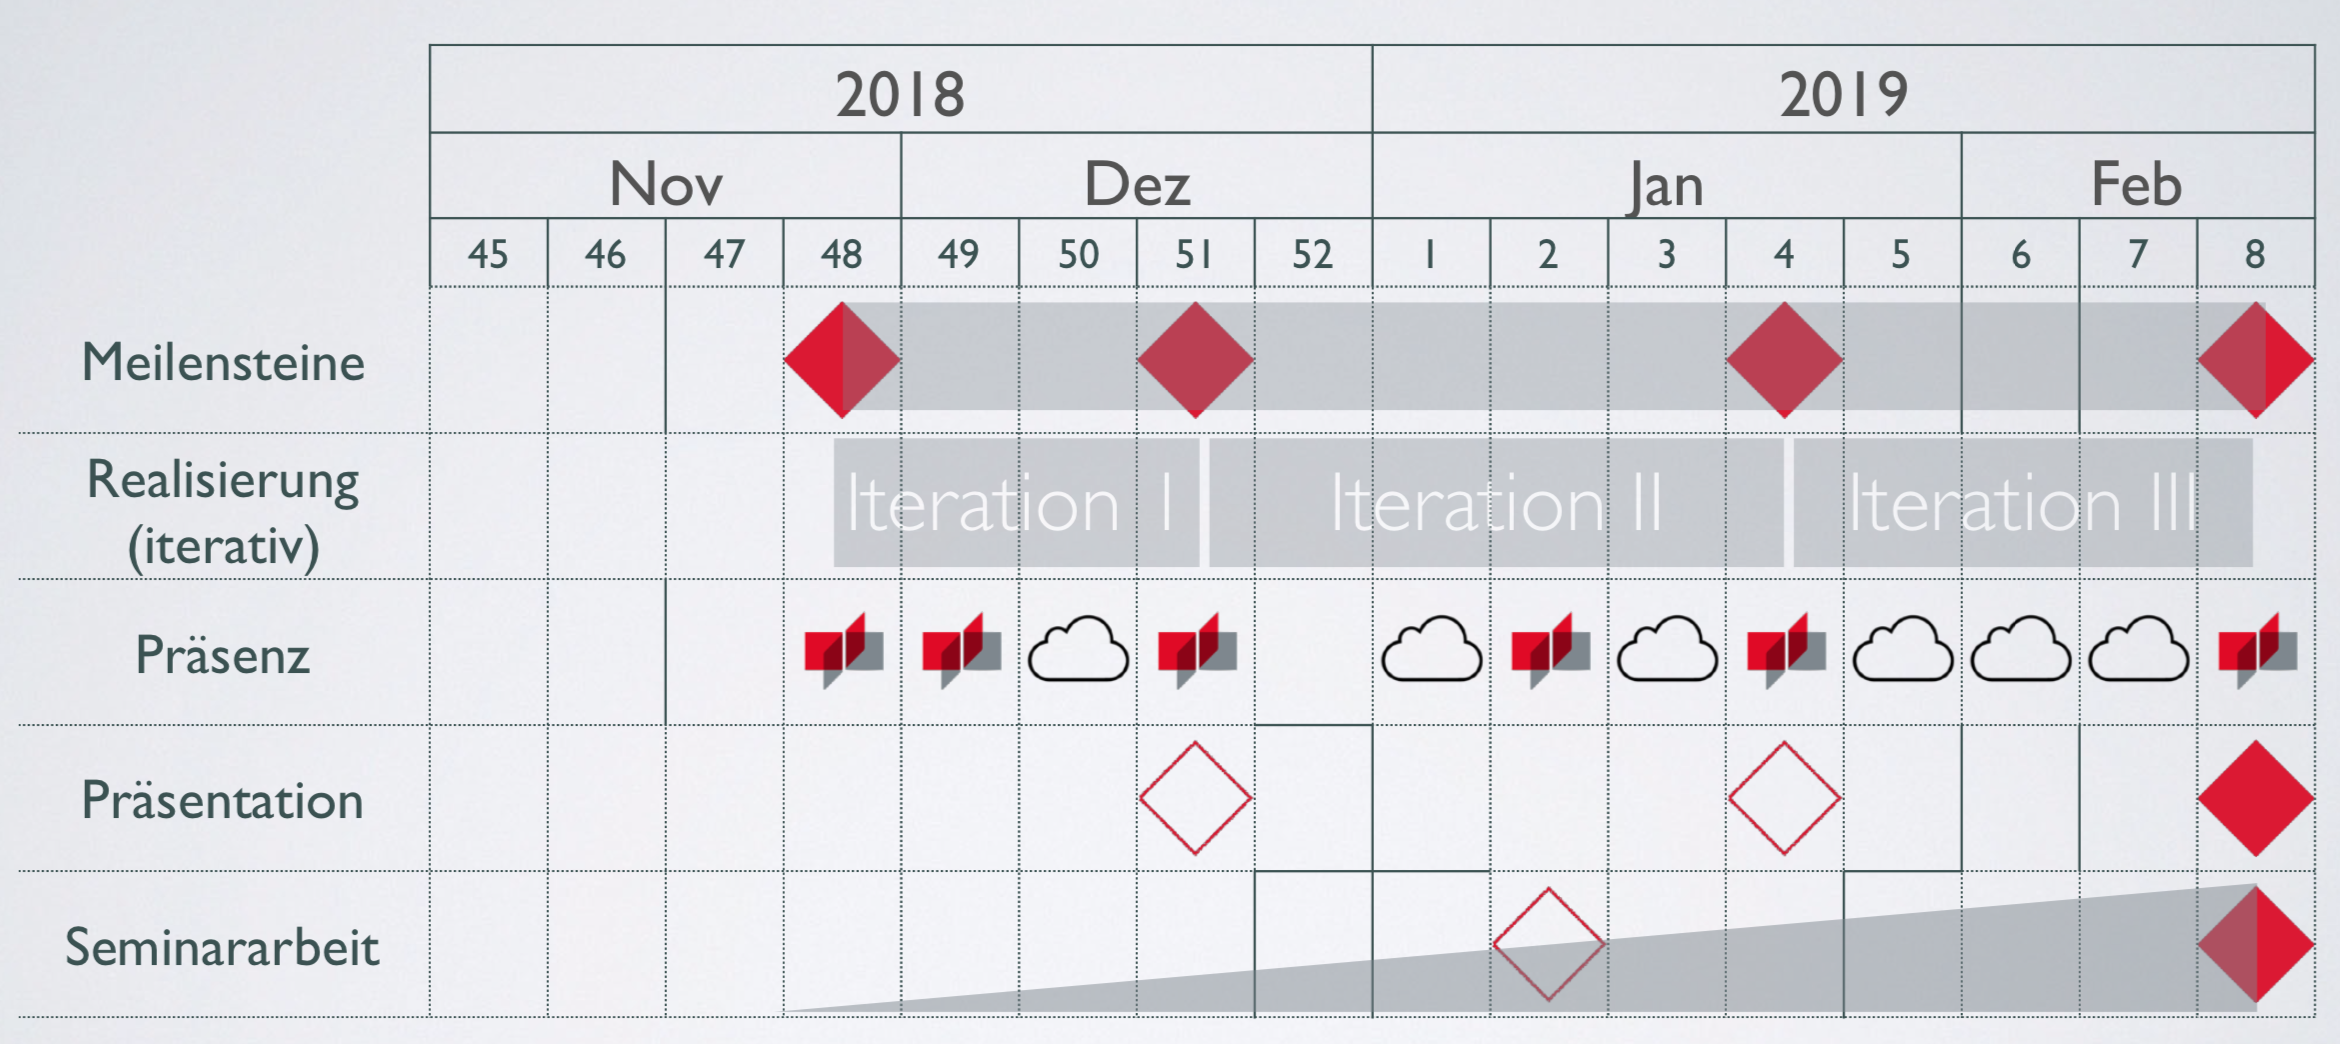
\includegraphics[width=12cm]{img/geplanterProjektablauf.png}
		\captionsetup{format=hang}
		\caption[Geplanter Projektablauf ]{\label{fig:projektablauf} Geplanter Projektablauf \\ Quelle: Skript, Gregor Tielsch }
	\end{figure}
	
	\subsection{Projektplanung mit Gantt Diagramm}
	Der Projektplan ist das zentrale Dokument des Projektmanagements, da er den Projektfortschritt unterstützt und alle Aufgaben enthält, die innerhalb dieses Projektes zu erledigen sind. Diese Dokumentation garantiert ein erfolgreiches und optimales Projektmangement. Das Gantt Diagramm ist eine Tabelle bestehend aus geplanten Vorgängen sowie Meilensteinen, die in einem dahinter dargestellten Kalender über Balken eingezeichnet werden\autocite[Vgl.][S. 107]{projektmanagement}. Heutzutage ist dieses Instrument des Projektmanagements die gängigste Methode, um Aktivitäten zeitbezogen zu dokumentieren. Um die Vorteile dieser Methode zu nutzen, wurde entschieden ein daran angelehntes Modell einzuführen. Damit der Projektplan jedem Teammitglied jederzeit zur Verfügung steht und um von der Nützlichkeit eines Online-Tools zu profitieren, wurde entschieden das Gantt Diagramm mit der Planungssoftware \enquote{Tom's Planner}\footnote{https://www.tomsplanner.de} zu erstellen.
	Das Projektmanagement wurde für die gesamte Projektzeit durchgeführt. Die Aktivitäten des Projekts sind in der Abbildung \vref{fig:projektplan} gruppiert dargestellt. Das Gantt Diagramm wurde stets während der Durchführung des Projektes gepflegt, um den aktuellen Projektfortschritt in einer übersichtlichen Darstellung zu visualisieren. In regelmäßigen Projektsitzungen wurde der Projektfortschritt über das Gantt Diagramm sowie die Meilensteile überwacht und dokumentiert. So ist der Projektstatus jederzeit transparent und für alle Teammitgliedern ersichtlich. Dadurch kann gegebenenfalls eingegriffen werden, wenn Meilensteine nicht erreicht werden und das Projekt in Gefahr läuft in Verzug zu geraten.  
	 Zu Beginn des Projektes wurden die Meilensteine in Orientierung an den Projektablaufplan Abbildung \vref{fig:projektablauf} angelegt. 
	\begin{figure}[H]
		\centering 
		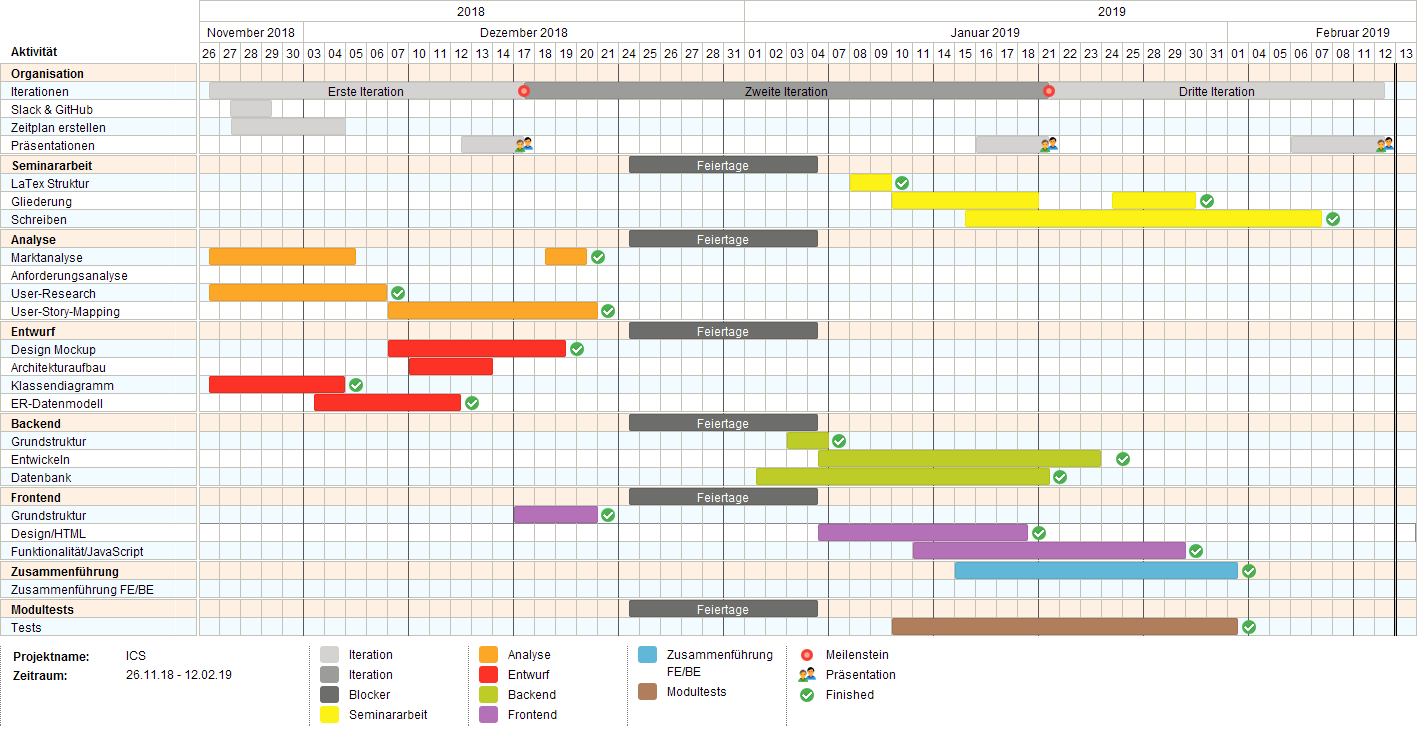
\includegraphics[width=14cm]{img/projektplan.png}
		\captionsetup{format=hang}
		\caption[Projektplan]{\label{fig:projektplan} Projektplan ICS, Gantt-Diagramm \\ Quelle: Tom's Planner}
	\end{figure}
	Die aktuell bearbeiteten Aufgaben wurden kontinuierlich in das Gantt Diagramm eingetragen, damit eine Übersicht entsteht, wann und wie lange an der jeweiligen Aufgabe gearbeitet wurde. Zunächst wurden einige organisatorische Aufgaben erledigt sowie ein Organisations-Tool eingerichtet. Die Organisation des Teams wird in Kapitel \vref{teamorga} genauer erläutert. Die Analyse (Kapitel \vref{analyse}) sowie der Entwurf (Kapitel \vref{entwurf}) wurden in der ersten Interation erarbeitet. Wobei die Marktanalyse in der zweiten Iteration erneut durchgeführt wurde, da zu diesem späteren Zeitpunkt neue Probleme aufgetreten sind. Nachdem das Grundkonzept der Anwendung durch ein Mockup und dem Design der Softwarearchitektur festgelegt wurde, konnte das Backend und das Frontend entwickelt. Dies wird im Kapitel \vref{umsetzung} detaillierter erklärt. In der zweiten und letzen Iteration wurde parallel zu der Entwicklung die Seminararbeit geschrieben. Gegen Ende der dritten Iteration wurde schließlich der Fokus auf die Präsentation sowie die Fertigstellung der Seminararbeit gelegt. Das Projekt endet am 12.02.2019 mit dem letzten Meilenstein \enquote{Abschlusspräsentation}.
	
	
	\section[Teamorganisation]{Teamorganisation{\hfill \normalsize Milena Zahn}} \label{teamorga}
	Eine wichtige Kompetenz innerhalb dieses Projektes ist es, sich selbst sowie das Team zu organisieren, um in dem begrenzten Zeitraum mit den gegebenen Resssourcen das Projektziel zu realisieren. Die Effizienz des Informationsaustausches und der Kommunikation innerhalb des Teams bestimmt wesentlich dessen Erfolg mit. Eine Hauptaufgabe in Projekten ist somit die Kommunikation\autocite[Vgl.][S. 207]{projektmanagement}. Insbesondere bei den zeitlich begrenzten Aufgaben und temporären Organisationsstrukturen ist ein reibungsloser Austausch, der jedes Projektmitglied mit den essentiellen Informationen versorgt, entscheidend. Aus diesem Grund wurde das Kommunikationstool \enquote{Slack}\footnote{https://slack.com/} gewählt. Die Projektbeteiligten sind alle mit dem Programm, unter anderem durch die Lernveranstaltung \textit{Systemanalyse und -entwurf} und durch die Praxisphasen in dem Unternehmen, vertraut. Dadurch kann eine Einarbeitungszeit eingespart werden kann. Für das Projekt wurde ein eigener Workspace, auf den alle Projektbeteiligten zugreifen können, angelegt. Kurze Teamabsprachen sowie Fragestellungen innerhalb des Teams, konnten damit schnell und unkompliziert geklärt werden. Ein weiterer Vorteil von Slack ist die Transparenz, die durch die verschiedenen, offenen Channels gegeben wird. Ein weiterer Vorteil ist die Dauerhaftigkeit der besprochenen Themen und beschlossenen Entscheidungen. Dadurch werden Entscheidungen dokumentiert und können bei Unklarheiten jederzeit wieder eingesehen werden. Durch \enquote{Slack} wurde damit ein stetiger, unkomplizierter Dialog unter den Teammitgliedern ermöglicht, der die Bearbeitung des Projektes unterstützt und vereinfacht hat.
	
	\section[Projektabschluss]{Projektabschluss{\hfill \normalsize Milena Zahn}} 
	Der Projektabschluss ist die letzte Phase für das Projekt. Es wird deutlich, ob die Ziele erreicht wurden und ein Projektreview erstellt. Dies wird in dem Kapitel \vref{Ausblick}, mit Fokus auf das Projektreview und Lessons Learned, und in dem Kapitel \vref{Evaluation}, mit Fokus auf die Zielerreichung und der Potenziale, ausgeführt. Das Projekt wird durch eine Abschlusspräsentation, in der der fertige Protoyp vorgestellt wird, sowie der vorliegenden Seminararbeit abgeschlossen. Die Projektabschlussbewertung wird schließlich von Herrn Gregor Tielsch, Dozent der Lehrveranstaltung \enquote{Fallstudie}, durchgeführt.
% !TEX root =  master.tex
\chapter{Methodik}
	Angewandte Methodik... agile und so (SCRUM, Sprints)
	
	iteratives Modell, warum kein Wasserfall
	
	Bei dem Wasserfallmodell werden die Phasen nur einmal in der vorgegeben Reihenfolge durchlaufen, bei dem iterativen Modell sind Rückspünge in vorherige Phasen vorgesehen. Somit lassen sich Änderungen, die erst zu einem späteren Projektzeitpunkt auftreten, mit in den Entwicklungsprozess berücksichtigt werden 
% !TEX root =  master.tex
\chapter{Analyse} \label{analyse}
	
%	\section{Anforderungsanalyse}
	
	\section[Ist-Analyse]{Ist-Analyse {\hfill \normalsize Yvonne Werner}}
	Mithilfe der Ist-Analyse wird eine bestehende Lösung zur Reservierung von Kinokarten betrachtet und evaluiert. Diese Betrachtung bildet die Grundlage für die Evaluierung der verschiedenen Aufbauten der Kinoreservierungssysteme. Dabei spielen vor allem die Verständlichkeit der Seite und die verschiedenen Schritte, die für eine Reservierung nötig sind, eine entscheidende Rolle. Außerdem wird verglichen, welche Schritte für die Reservierung notwendig sind, mit den verschiedenen Seiten, auf die man weitergeleitet wird. Dabei wird versucht herauszufinden, welche Funktionen für eine Reservierung essenziell sind und welche zusätzliche Funktionen darstellen. Des Weiteren werden die verschiedenen Möglichkeiten einer Bestätigung sowie die Notwendigkeit eines Benutzerkontos betrachtet. 
	
	\subsection{Kinopolis Viernheim}
	Beim Öffnen der Seite fällt auf, dass das Hauptfenster zur Reservierung von Karten von einem Rahmen mit Werbung für einen aktuellen Film umgeben ist (siehe Abb. \vref{fig:Kinop.Start}). Nach dem Klicken auf diesen Teil der Seite, wird der Nutzer zu einer Übersichtsseite dieses Films weitergeleitet. 
	\begin{figure}[H]
		\centering 
		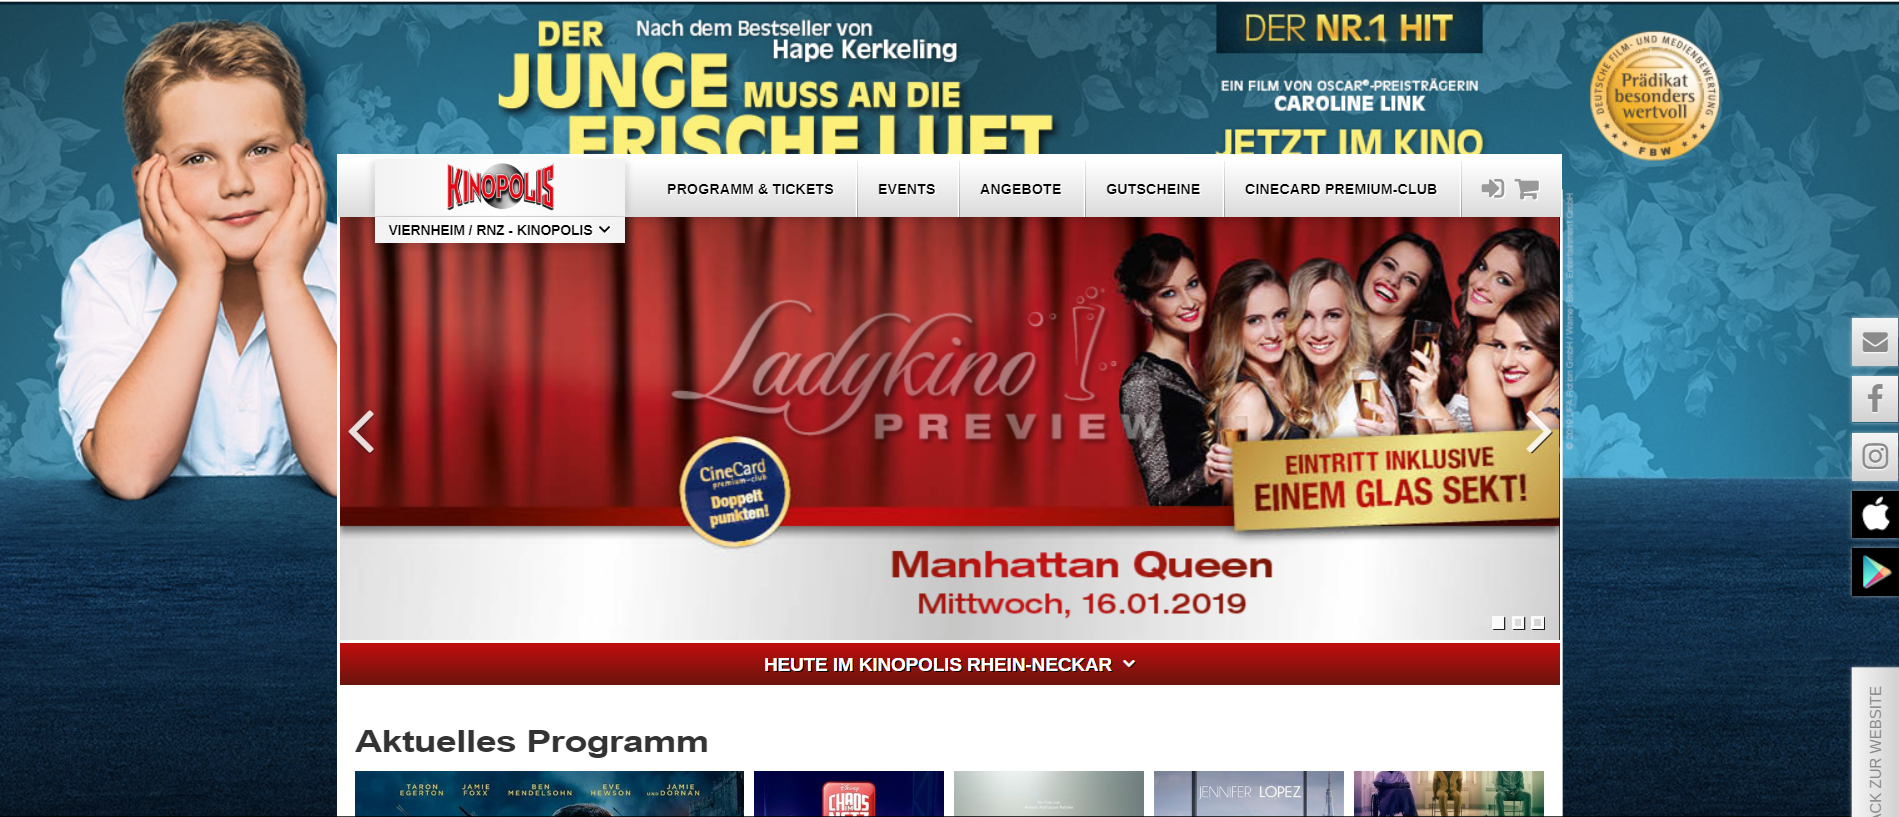
\includegraphics[scale=0.38]{img/Kinopolis_MA_Startseite.png}
		\captionsetup{format=hang}
		\centering\caption[Startseite von Kinopolis Viernheim]{\label{fig:Kinop.Start}Startseite von Kinopolis\footnotemark}
	\end{figure} \footnotetext{Quelle: https://www.kinopolis.de/vi}

	Die eigentliche Hauptseite in der Mitte enthält eine Kopfleiste, in der zwischen Programm \& Tickets sowie zwischen Events, Angeboten und Gutscheinen gewählt werden kann. Außerdem besteht die Möglichkeit, sich für eine Premium-Club Card zu registrieren, um Punkte sammeln und diese in Vorteile umwandeln zu können. Des Weiteren ist über ein Symbol die Anmeldung zu einem eingerichteten Account möglich. Unterhalb des Kopfs informiert eine Leiste mit wechselndem Inhalt über Events zu aktuellen Filmen. Als Beispiel wird unter anderem eine \enquote{Ladykino Preview} und ein sich bewegender Sitz angepriesen. 
	\\Nachfolgend findet der Nutzer unter der Überschrift \enquote{Aktuelles Programm} einige ausgewählte Filme. Sie werden in der Plakatansicht dargestellt (siehe Abb. \vref{fig:Kinop.Start2}), weshalb für den Nutzer auf den ersten Blick nur das Filmplakat und der Titel ersichtlich sind. Mithilfe des darunterliegenden Buttons können weitere aktuelle Filme angezeigt werden. Durch das Führen der Maus auf das Plakat eines Films, ergibt sich die Auswahl zwischen dem Anschauen des Trailers, dem Lesen von Filminformationen und dem direkten Kauf von Tickets über die Auswahl der Vorstellung.
	\begin{figure}
		\centering 
		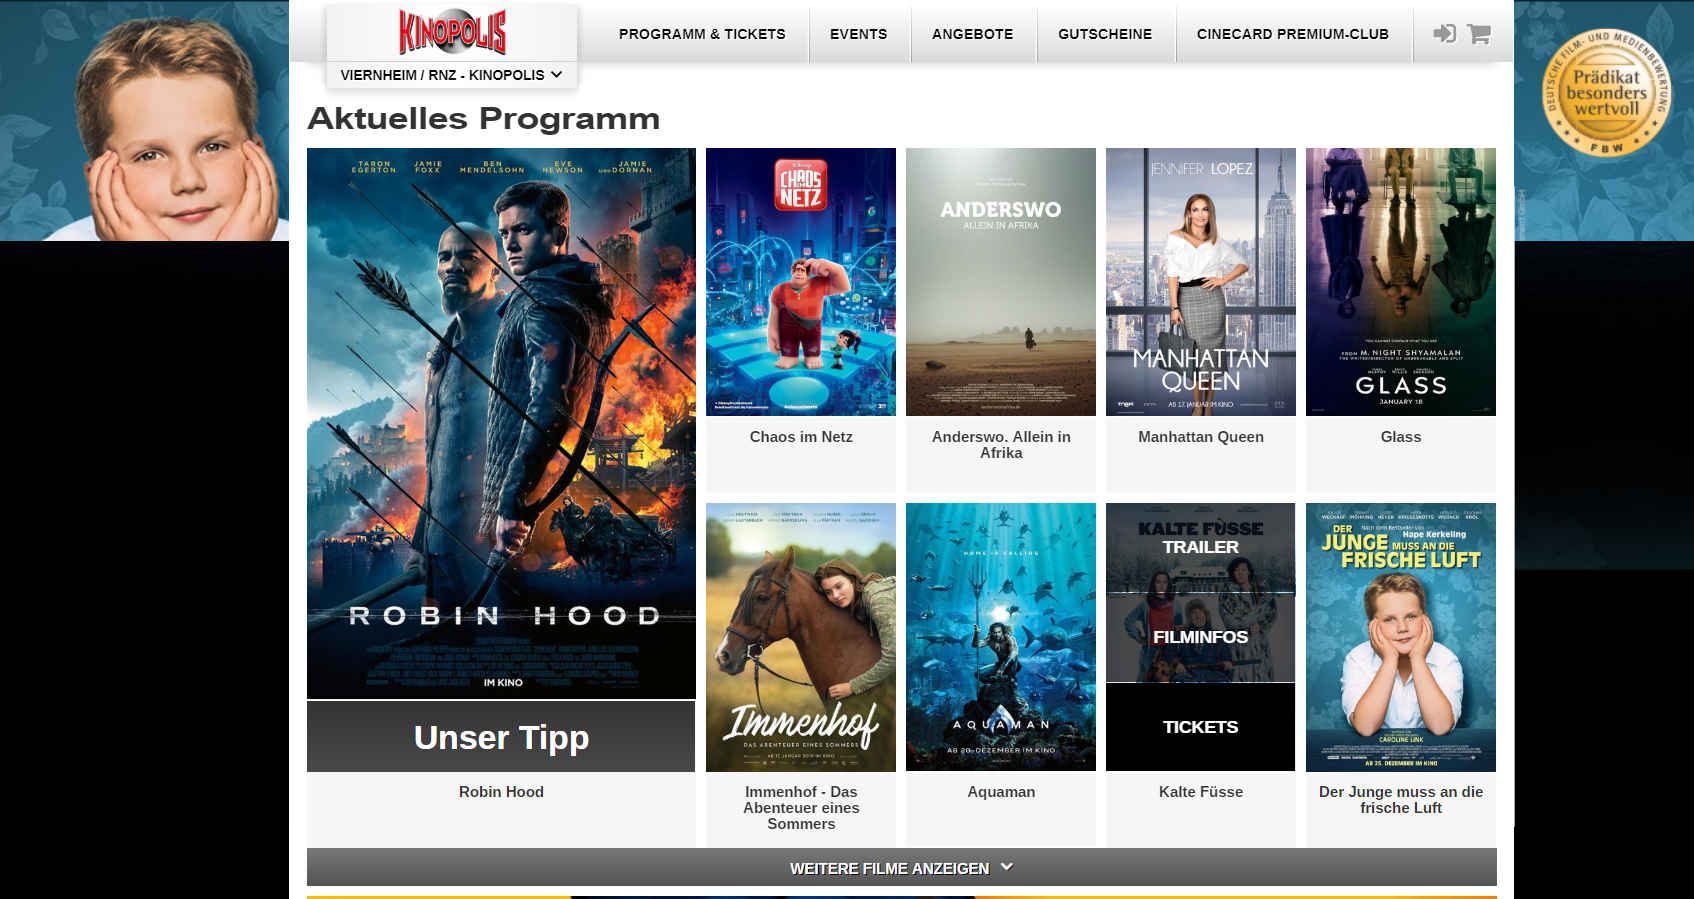
\includegraphics[scale=0.38]{img/Kinopolis_MA_Start2.png}
		\captionsetup{format=hang}
		\centering\caption[Startseite von Kinopolis Viernheim]{\label{fig:Kinop.Start2}Startseite von Kinopolis\footnotemark}
	\end{figure}
	\footnotetext{Quelle: https://www.kinopolis.de/vi}
	Neben diesen Bereichen enthält die Startseite von Kinopolis ebenfalls Informationen zu aktuellen Events, wie \enquote{Kids Previews} und \enquote{Ladykino}. Darüber hinaus bieten sich darunter befindende Abschnitte Auskunft zu Filmen, die bald anlaufen werden, sowie Nachrichten aus Hollywood. 
	
	Die zweite Möglichkeit zur Auswahl eines Filmes besteht durch den zweiten Tab \enquote{Programm \& Tickets}. Dort befindet sich zunächst eine Leiste, in der die Vorstellungen für einen bestimmten Tag oder für eine ganze Woche angezeigt werden können. Standardmäßig ist die Übersicht einer Woche ausgewählt (siehe Abb.\vref{fig:Kinop.Progr.}), wodurch zu jedem Film alle Vorstellungen der Woche aufgelistet sind. Neben der zeitlichen Eingrenzung der Suche, können mit dem in der Abbildung ausgeklappten Programmfilter weitere Eingrenzungen erfolgen. Die Filterung kann nach Genre, FSK-Stufen, Art der Darstellung (2D, 3D, ...) und nach zeitlicher Eingrenzung eines Tages erfolgen. Durch die zuletzt genannte Filtermöglichkeit, wird der Beginn der Vorstellungen in Vormittags, Nachmittags und Abends eingestuft.
	\\Rechts neben dem Programmfilter kann je nach Präferenz des Nutzers zwischen zwei Ansichten für die Auflistung der Filme gewechselt werden. Zur Auswahl steht die Listenansicht, sowie die Plakatansicht. Voreingestellt ist die Listenansicht, in der die Filme untereinander dargestellt werden. Zu jedem Film sind Eckdaten wie beispielsweise das Genre, die Länge, und der Start (die erste Vorstellung dieses Films) angegeben. Außerdem wird durch Labels unterstützend ersichtlich, welche FSK-Stufe für den Film besteht. Zusätzliche Labels unterrichten den Nutzer über spezielle Events sowie Angebote. Des Weiteren wird ein Überblick über die Vorstellungen eines Films der kommenden Woche geboten. Dabei wird neben der Zeit ebenfalls der Saal angegeben. Durch das Überfahren einer Vorstellung mit der Maus bekommt der Nutzer die Eckdaten des jeweiligen Saals angezeigt. Bei speziellen Anforderungen an den Saal, kann der Nutzer über den Button \enquote{Saalübersicht} die Daten zu allen vorhandenen Sälen abrufen und somit viel Zeit bei der Suche nach einem Kinosaal, der die Anforderungen erfüllt, sparen. Im nächsten Schritt kann der Nutzer entweder weitere Informationen zu einem Film anschauen, indem er auf den Button \enquote{Filminfos} oder auf den Titel klickt. Dadurch wird der Nutzer auf eine Detailseite weitergeleitet, die im nachfolgend erläutert wird. Wenn der Nutzer bereits eine Vorstellung ausgewählt hat, bekommt er durch das Anklicken der Vorstellung auf die Reservierungsseite weitergeleitet. 
	\\Die Plakatansicht als zweite Möglichkeit der Darstellung ist ähnlich aufgebaut, wie die Darstellung der Filme auf der Startseite. Der Nutzer sieht die verschiedenen Filmplakate und den Titel dieser. Es liegt also an dem Nutzer, ob er zusätzliche Informationen zu dem Film direkt ersichtlich haben möchte oder nicht.  
	\\Neben den zwei erklärten Seiten, bietet das Portal weitere Seiten mit Informationen über Events, Angebote und anderen Vorteilen, die nicht zwingend zur Reservierung von Karten notwendig sind. Deshalb werden diese Seiten in der Ist-Analyse zwar registriert, aber nicht als essenzielle Anforderungen an ein Kinoreservierungssystem erfasst. Aus diesem Grund werden sie nicht näher erläutert.
	\begin{figure}
		\centering 
		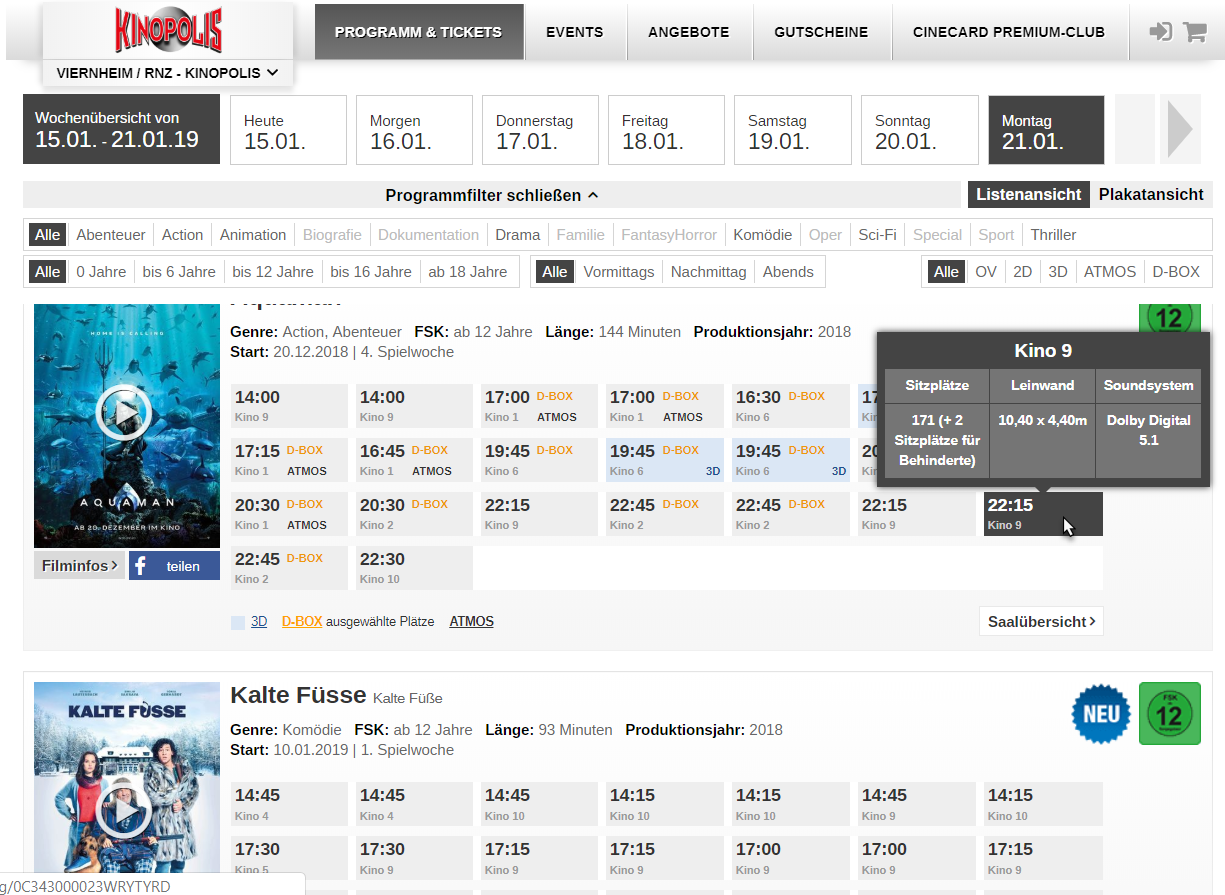
\includegraphics[scale=0.45]{img/Kinopolis_Programm_Tickets.png}
		\captionsetup{format=hang}
		\centering\caption[Startseite von Kinopolis Viernheim]{\label{fig:Kinop.Progr.}Programm \& Tickets von Kinopolis\footnotemark}
	\end{figure}
	\footnotetext{Quelle: https://www.kinopolis.de/vi}
	
	Eine weitere Unterstützung zur Auswahl eines Kinofilms bietet die Detailseite, die einen Überblick über Trailer, die wichtigsten Informationen und die verschiedenen Vorstellungen bietet. Der Nutzer kann die  Detailseite erreichen, indem er auf der Startseite, nach Positionierung der Maus über dem gewünschten Filmplakat, auf die Option Filminfos klickt. Ein solcher Button befindet sich auch in der Seite Programm \& Tickets unterhalb des Trailers. Zusätzlich dazu kann auch der Nutzer über den Filmtitel auf die Detailseite navigieren. 
	\\Dort werden zunächst verschiedene Videos zur Auswahl gestellt. Darunter befindet sich der Trailer und je nach Film weitere Videos, wie beispielsweise das Making-Of. Des Weiteren kann der Nutzer das Filmplakat und eine Bewertung nach 5-Sterne-System sehen und auch selbst abgeben. Über die Eckdaten des Films gelangt der Nutzer in einen Bereich, indem der Inhalt des Film geschildert wird. Dieser ist in deutsch, sowie in einem anderen Tab auch in englisch vorhanden. Ein dritter Tab führt zu Bildern von verschiedenen Szenen des Films. Der darunterliegenden Bereich zeigt eine Übersicht der Vorstellungen für die nächsten sieben Tage. Jede Vorstellung enthält die Startzeit, den Saal, sowie das Vorhanden sein von speziellen Sitzen und ob der Film in 3D läuft. Als Nächstes wird die Besetzung des Films aufgeführt. Dazu werden die wichtigsten Schauspieler des Films mit ihren Namen und einem Foto gezeigt.  
	
	Wenn sich der Nutzer für eine bestimmte Vorstellung entschieden hat, gelangt er durch das Anklicken dieser Vorstellung zur Reservierungsseite. Die Auswahl der Vorstellung kann in der zuletzt vorgestellten Detailseite über die angezeigten Vorstellungen der nächsten Woche, sowie über die Seite \enquote{Programm \& Filme} und die Startseite durch das Anklicken von \enquote{Tickets} erfolgen. 
	\\Die nachfolgende Seite enthält die Möglichkeit der Platzauswahl in dem jeweiligen Kinosaal der Vorstellung. Es wird nochmals das Filmplakat gezeigt, wodurch sich der Nutzer sich sein kann, die Karten für den gewünschten Film auszuwählen. Zusätzlich wird das Datum und die Uhrzeit der Vorstellung angegeben, wodurch eine Verwechslung ausgeschlossen ist.
	Nachfolgend kann der Nutzer entscheiden ob er die Karten kaufen oder reservieren möchte, mit dem Unterschied, dass bei einem Kauf der Karten ermäßigte Tickets für Kinder, Schüler, Studenten und Senioren gekauft werden können. Bei einer Reservierung wird nur die Anzahl der Karten ausgewählt und eventuelle Ermäßigungen müssen an der Kasse besprochen werden. Außerdem muss bei verschiedenen Preiskategorien der Plätze neben dem Wählen der Anzahl auch die Kategorie der Sitzplätze gewählt werden, damit nachfolgend nur Plätze der gewünschten Kategorie gewählt werden können. 
	Wenn der Nutzer eine bestimmte Anzahl ausgewählt hat, kann er mithilfe eines visualisierten Sitzplans seine bevorzugten Plätze wählen. Die Abbildung enthält die Position der Leinwand, den Eingang und die Treppen des Saals. Jeder Sitz des Raums ist eingezeichnet und enthält durch seine Darstellung Informationen über den Buchungsstatus. Durch die farblich verschiedenen Plätze kann der Nutzer die Preiskategorien voneinander unterscheiden, sowie auf einen Blick erkennen, welche Plätze bereits belegt und welche Plätze nicht buchbar sind. 
	\\Hat sich der Nutzer für bestimmte Plätze entschieden, so kann er diese in der Platzkarte auswählen. In diesem Reservierungssystem können nur Plätze nebeneinander gebucht werden, wodurch die Anzahl der ausgewählten Plätze immer nebeneinander liegt. Dadurch wird versucht einzelne buchbare Sitze zwischen gebuchten Sitzen zu vermeiden. Nach der Platzwahl kann ein Nutzer die Karten kaufen bzw. reservieren. 
	
	Dazu gelangt er über einen erscheinenden Button zunächst auf eine Seite, die einen Überblick über die gewählten Produkte gibt. Der Nutzer kann sich entscheiden, ob er die Karten mit vorhandenem Kundenkonto über einen Login oder als Gast kaufen bzw. reservieren möchte. Außerdem besteht die Möglichkeit ein neues Nutzerkonto anzulegen. Bei der Wahl des Gastzugangs wird der Nutzer aufgefordert seinen Namen, sowie E-Mail und Geburtsdatum anzugeben. 
	Beim Reservieren von Karten können die Karten durch den Button \enquote{Jetzt reservieren} reserviert werden, wodurch der Nutzer eine Reservierungsnummer als Bestätigung zugewiesen bekommt. Mit dieser kann er die Karten bis eine halbe Stunde vor Beginn der Vorstellung an der Kasse abholen. Auf der Bestätigungsseite bekommt der Nutzer ebenfalls die Möglichkeit die Reservierung zu drucken, sodass er sie auch ausdrucken könnte. Des Weiteren hat der Kunde die Möglichkeit die Karten zu kaufen oder direkt zu stornieren. 
	\\In dem Kaufvorgang gelangt der Kunde nach dem Anklicken von \enquote{Weiter} in die Ansicht des Warenkorbs, welche die wichtigsten Informationen zu der Vorstellung und dem Standort des Kinos enthält. Außerdem werden Reihe und Plätze der Sitze mit ihrem dazugehörigen Preis angezeigt. Danach muss die Zahlungsmethode gewählt werden, wobei die verschiedenen Auswahlmöglichkeiten zunächst schwer zu erkennen sind. Nach der Auswahl werden die Tickets bezahlt und der Kunde kann in dem Kino direkt reingehen ohne sich zuvor an der Kasse anstellen zu müssen. 
	
	\begin{center}
		\textbf{Bilder von Detailsseite?; von Auswahl der Sitze; Reservierungsansicht}
	\textbf{\\Text dazuschreiben, warum nur die Bilder der Reservierung genommen werden?}
	\end{center}
	
	\subsubsection{Zusammenfassung der erforderlichen Schritte} 
	Für eine Reservierung von Karten sind vier Schritte von Bedeutung. Zunächst muss sich der Nutzer für einen Film entscheiden. Dies kann durch den Trailer oder das Lesen der Filmbeschreibung geschehen. Nachfolgend wählt der Kunde einen Tag und eine Uhrzeit aus, an dem er sich den Film anschauen möchte. In dem nächsten Schritt entscheidet er sich für eine bestimmte Anzahl an Plätzen sowie wo sich die Sitze in dem Kinosaal befinden sollen. Als letzter Schritt erfolgt die Reservierung der Tickets indem der Kunde seine Daten angibt und dadurch eine Reservierungsnummer mitgeteilt bekommt, mit der er die Karten im Kino abholen kann.
	
	\section[Soll-Analyse]{Soll-Analyse {\hfill \normalsize Milena Zahn}}
		
	 	\subsection{User-Research-Prozess} 
	 	User Research ist eine systematische Untersuchung der Ziele, Bedürfnisse und Fähigkeiten der Benutzer\autocite[Vgl.][S. 6]{Schumacher.2010}.
	 	Durch diesen Prozess lässt sich sicherstellen, dass die entwickelte Software den Nutzern einen Mehrwert bietet und an deren Bedürfnisse angepasst ist.
		Der Prozess startet mit der Definition der \textit{User Profile}. Diese klassifizieren Endanwender mit Nutzerprofilen, damit eine konkrete Vorstellung der Anwender geschaffen wird. Anhand von detaillierten Beschreibungen von Attributen lässt sich die Nutzergruppe identifizieren.
		
		\begin{table}[H]
			\centering
			\begin{tabular}{p{5,5cm} || c | c }
				\textbf{Attribute} & \textbf{Endanwender} & \textbf{Mitarbeiter} \\\toprule
				Alter &  16 - 99 Jahre &  16 - 99 Jahre \\
				Geschlecht &  männlich und weiblich &  männlich und weiblich  \\
				Medienkompetenz &  ja und nein &  ja  \\
				Erfahrung Onlinereservierung &  ja und nein &  ja  \\
			\end{tabular}
			\caption[User Profile]{\label{tab:tabelleUserProfile}User Profile}
		\end{table}
		
		Im nächsten Schritt werden Personas aus den User Profiles erstellt. Personas sind fiktive Personen, die für eine Nutzergruppe steht. Der Zweck von Personas ist, dass Entwickler Empathie und Einfühlungsvermögen zu den konkreten Anwendern aufbauen können. 
		
		\begin{figure}[H]
			\subfigure[Persona Franzi]{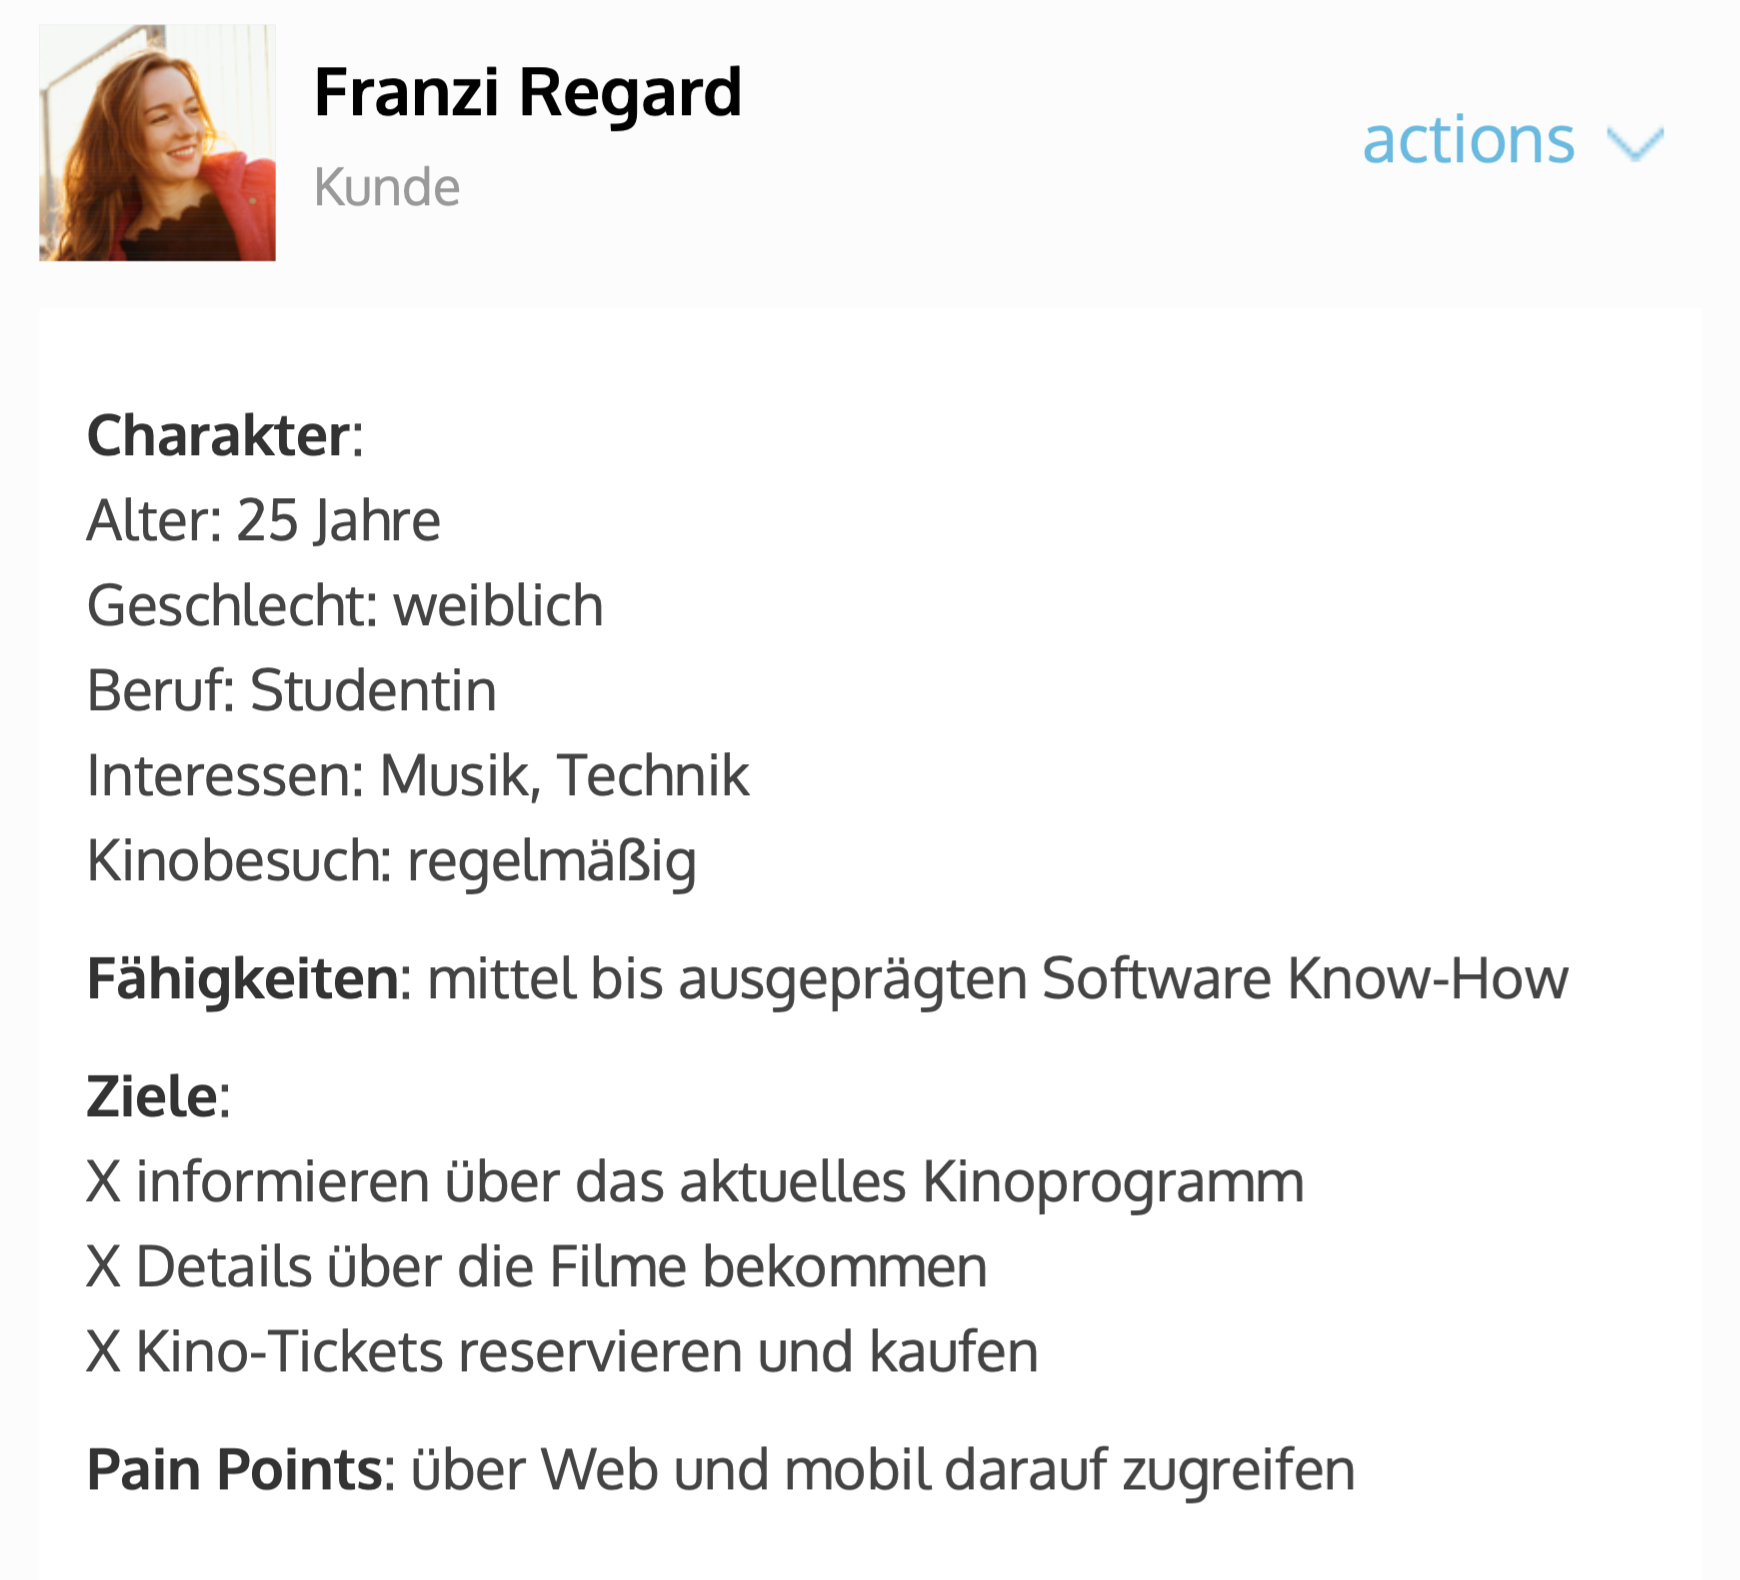
\includegraphics[width=0.49\textwidth]{img/franzi.png}} 
			\subfigure[Persona Gustav]{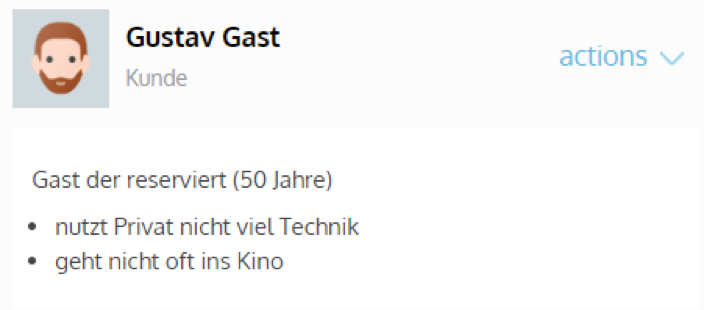
\includegraphics[width=0.49\textwidth]{img/gustav.png}} 
			\subfigure[Persona Kassandra]{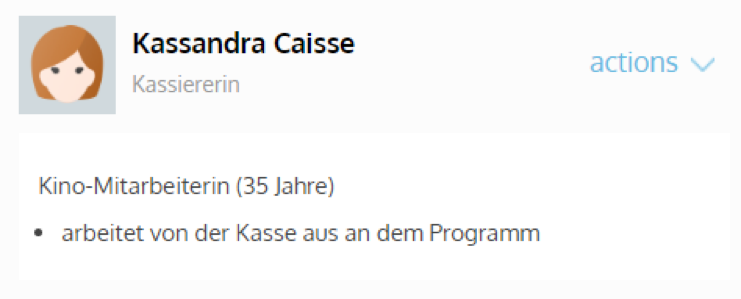
\includegraphics[width=0.49\textwidth]{img/kassandra.png}} 
			\subfigure[Persona Walter]{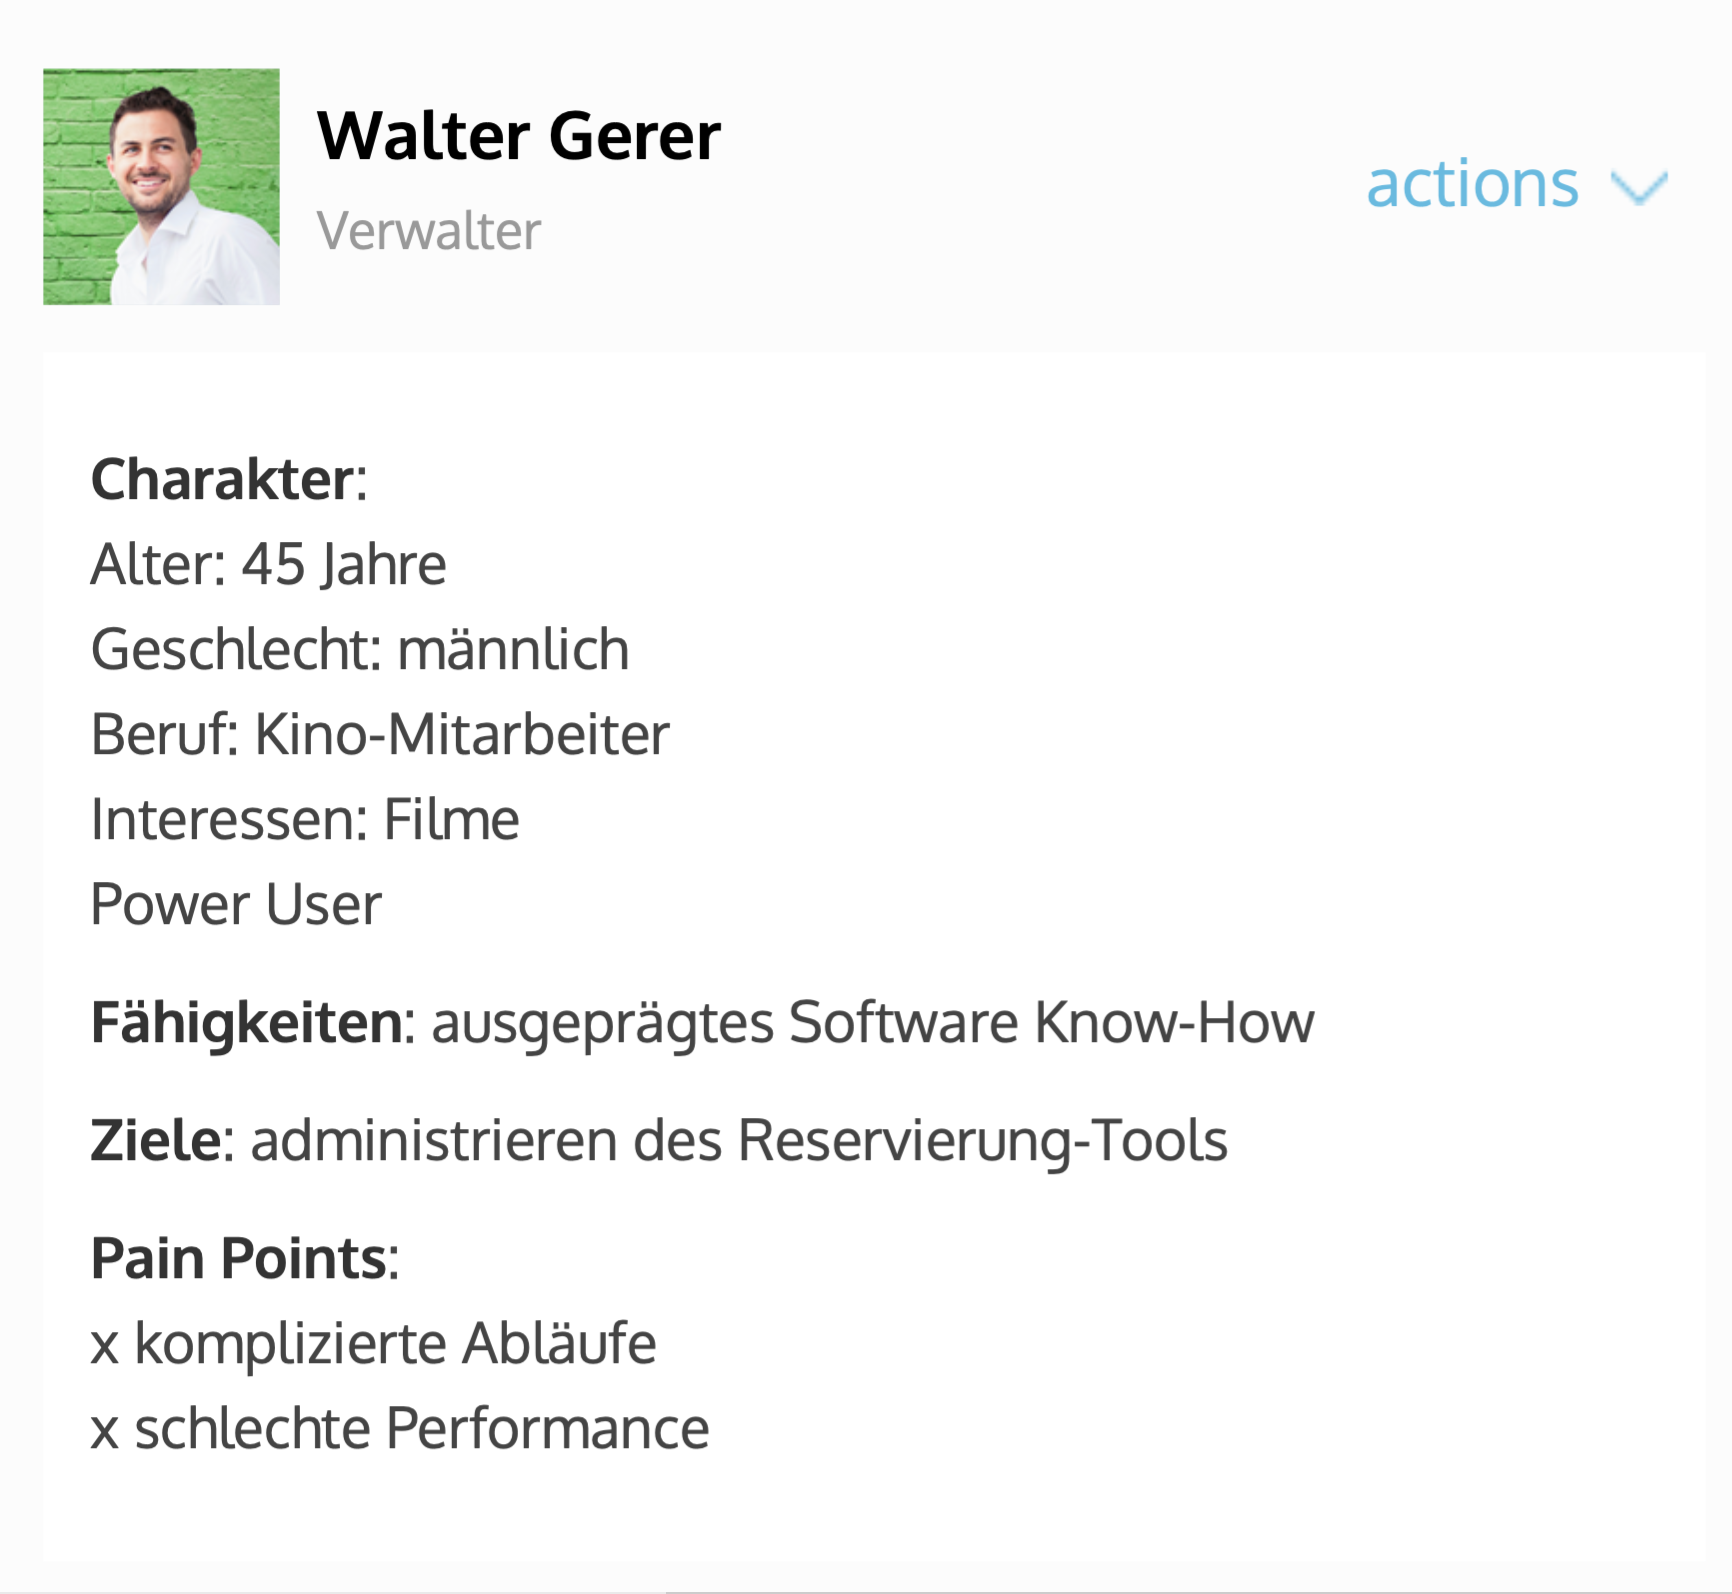
\includegraphics[width=0.49\textwidth]{img/walter.png}} 
			\caption[Personas ]{\label{fig:personas}Personas [DRAFT - detaillierter!] }
		\end{figure} 
		
		Darauf aufbauend werden Use Cases für die Personas entwickelt. Diese beschreiben Szenarien, wie die Personas das Endprodukt verwenden werden und welche Vorgehensweisen und Anforderungen dabei haben. 
		
		\begin{figure}[H]
			\begin{tabular}{p{13cm}}
				\textbf{Franzi Regard} \\\toprule
				Als Franzi möchte ich mich schnell vom meinem Smartphone oder Laptop aus über das aktuelle Kino-Programm informieren und Kino-Tickets reservieren und kaufen, um mit meinen Freunden einen Film anzuschauen. Dabei lege ich viel Wert auf ansprechendes Design und eine schnelle Abwicklung.
			\end{tabular}
			\caption[Use Case Franzi]{\label{fig:useCaseFranzi} Use Case Franzi [DRAFT]}
		\end{figure}
	
		\begin{figure}[H]
			\begin{tabular}{p{13cm}}
				\textbf{Gustav Gast} \\\toprule
				Als Gustav möchte ich Kino-Tickets reservieren, um mit meiner Familie einen Familienabend zu verbringen. Eine intuitive Anwendung ist für mich sehr wichtig, weil noch nie online Tickets reserviert habe. 
			\end{tabular}
			\caption[Use Case Gustav]{\label{fig:useCaseGustav} Use Case Gustav [DRAFT]}
		\end{figure}
	
		\begin{figure}[H]
			\begin{tabular}{p{13cm}}
				\textbf{Kassandra Caisse} \\\toprule
				Als Kassandra möchte ich mir die Reservierungen anschauen und Reservierungen anpassen können. 
			\end{tabular}
			\caption[Use Case Kassandra]{\label{fig:useCaseKassandra} Use Case Kassandra [DRAFT]}
		\end{figure}

		\begin{figure}[H]
			\begin{tabular}{p{13cm}}
				\textbf{Walter Gerer} \\\toprule
				Als Walter möchte ich das Kino-Programm verwalten und einpflegen. 
			\end{tabular}
			\caption[Use Case Walter]{\label{fig:useCaseWalter} Use Case Walter [DRAFT]}
		\end{figure}
		
	\subsection{User-Story-Mapping}
	Schließlich wird aus den Personas das User-Story-Mapping erstellt. In dieser werden die aus den Use-Cases hervorgehenden Features visuell geplant und in unterschiedliche Releases priorisiert. 

	%Stories On Board erklären
	%Usm erläutern
	\begin{figure}[H]
		\subfigure[Teil 1]{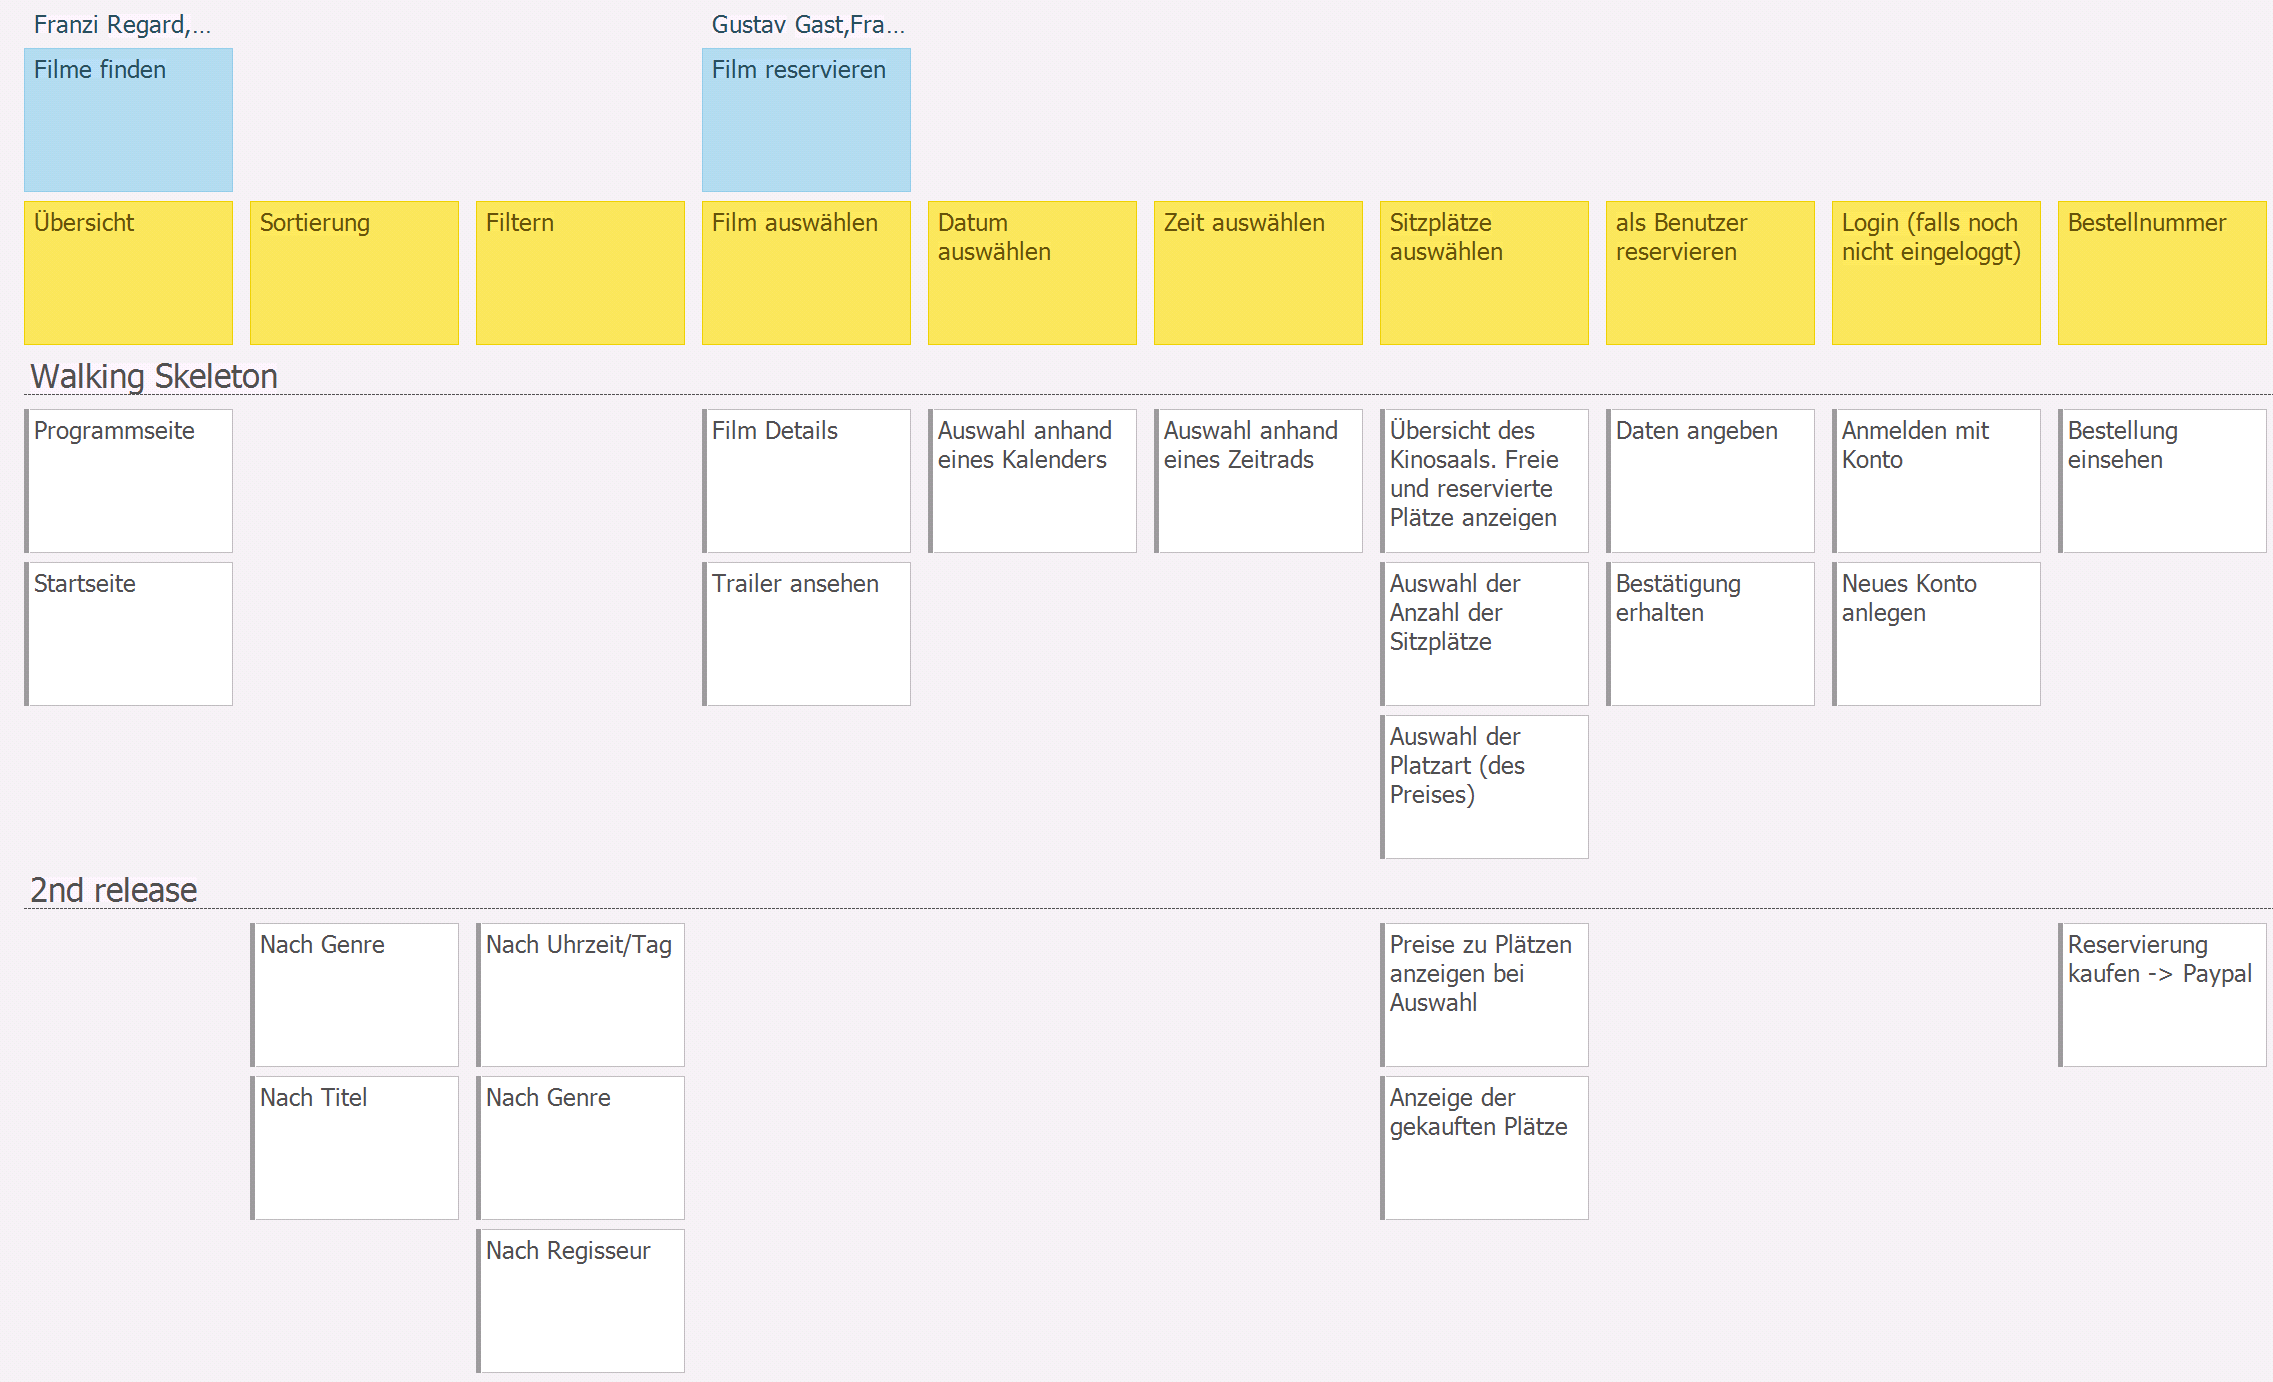
\includegraphics[width=14cm]{img/usm1.png}} 
		\subfigure[Teil 2]{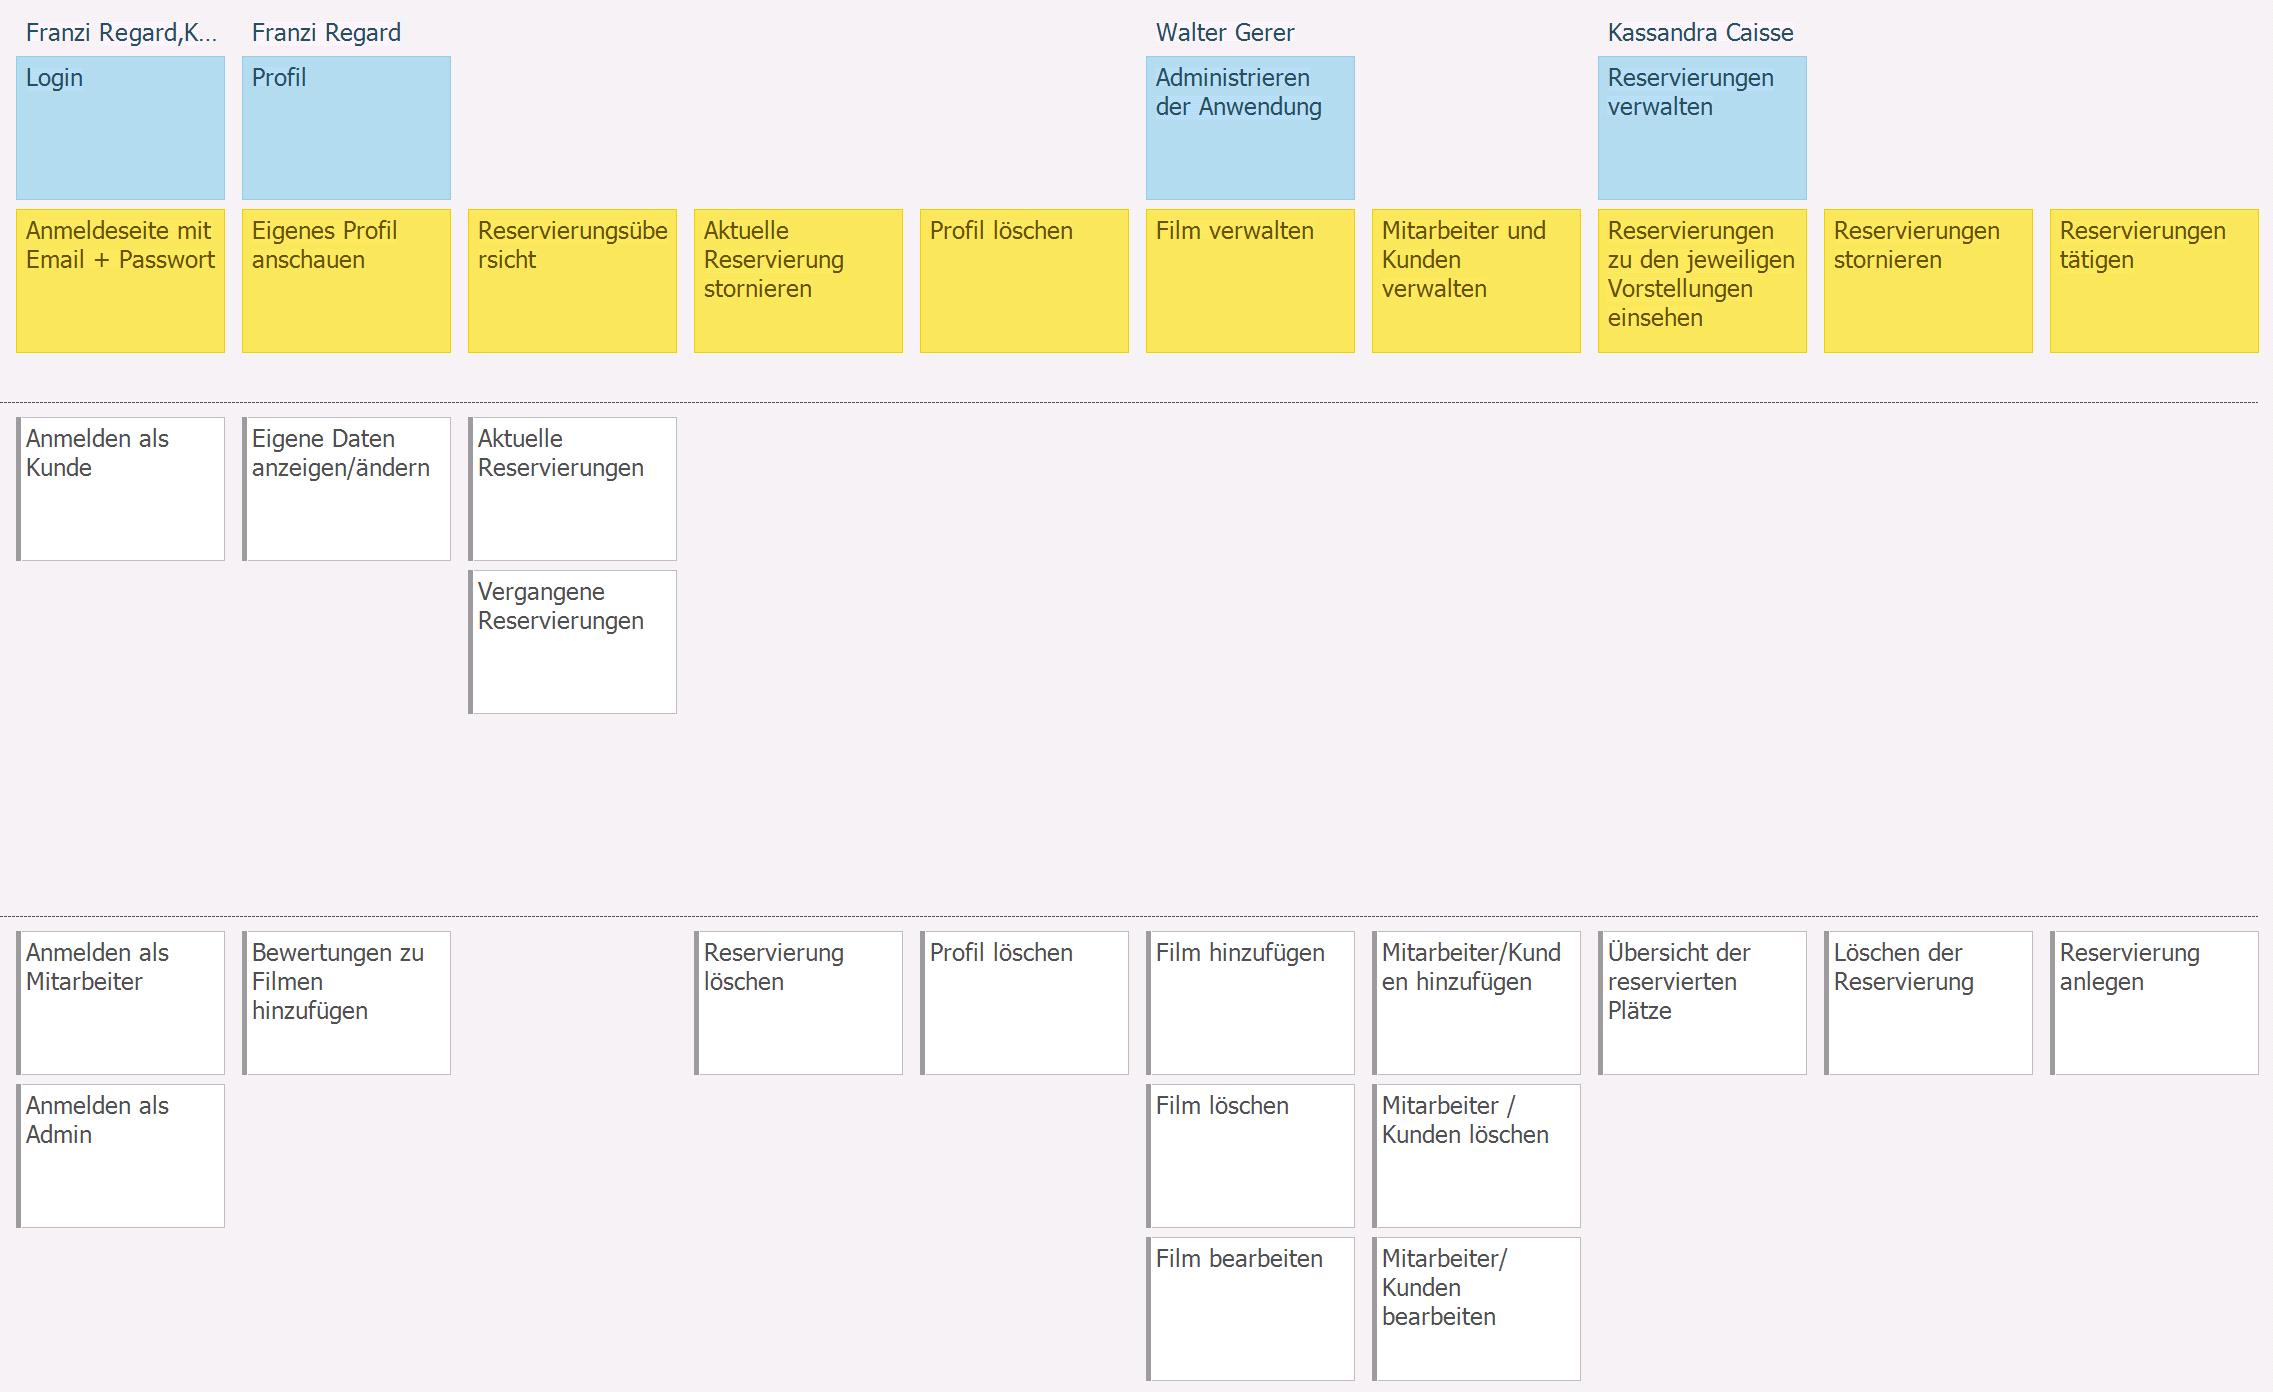
\includegraphics[width=14cm]{img/usm2.png}} 
		\caption[User-Story-Map ]{\label{fig:userStoryMap}User-Story-Map\\ Quelle: Stories on Board}
	\end{figure} 
	 	
%		\subsection{Vorgabe}
%		\subsection{Rahmenbedingungen}
%		\subsection{Bewertungskriterien}
% !TEX root =  master.tex
\chapter{Entwurf}\label{entwurf}
	\section[Design Entwurf]{Design Entwurf {\hfill \normalsize Dennis Köhler}}\label{design}
		
		Damit eine klare Struktur für die Frontend Entwicklung gegeben ist und mehrere Entwickler auf gleichem Wissensstand mit dem Programmieren beginnen können ist ein Entwurf essentiell. Der Design Entwurf stellt die erste konkrete Idee für das Frontend dar und wurde auf Basis der Analyse marktführender Kinowebseiten erstellt. Er soll nicht als strenge Richtlinie für die Umsetzung verstanden werden, sondern ist vielmehr als Orientierungshilfe und Unterstützung zu verstehen. Die wichtigsten Unterschiede zur realisierten Umsetzung werden später im Abschnitt \vref{subdesign} dargestellt. 
		
		Der Entwurf wurde in einem kleineren Team mithilfe diverser Zeichenapps auf dem iPad erstellt. Auch wenn eine Reihe an Tools wie \enquote{Mockingbird} oder \enquote{wireframe.cc} für genau diesen Anwendungsfall gedacht sind, wurde sich bewusst dagegen entschieden. Gründe hierfür sind zum Beispiel die benötigte Einarbeitungszeit in das entsprechende Tool oder deren reduzierter Funktionsumfang in kostenlosen Testversionen. 
		Als Mockup dargestellt wurden die drei Hauptseiten: Startseite, Programm und Sitzplan, welche den Funktionsumfang des Reservierungsprozesses enthalten, abbilden. Die Startseite ist in Abbildung \ref{fig:mockUpStartseite} zu sehen.
		
		\begin{figure}[H]
			\centering 
			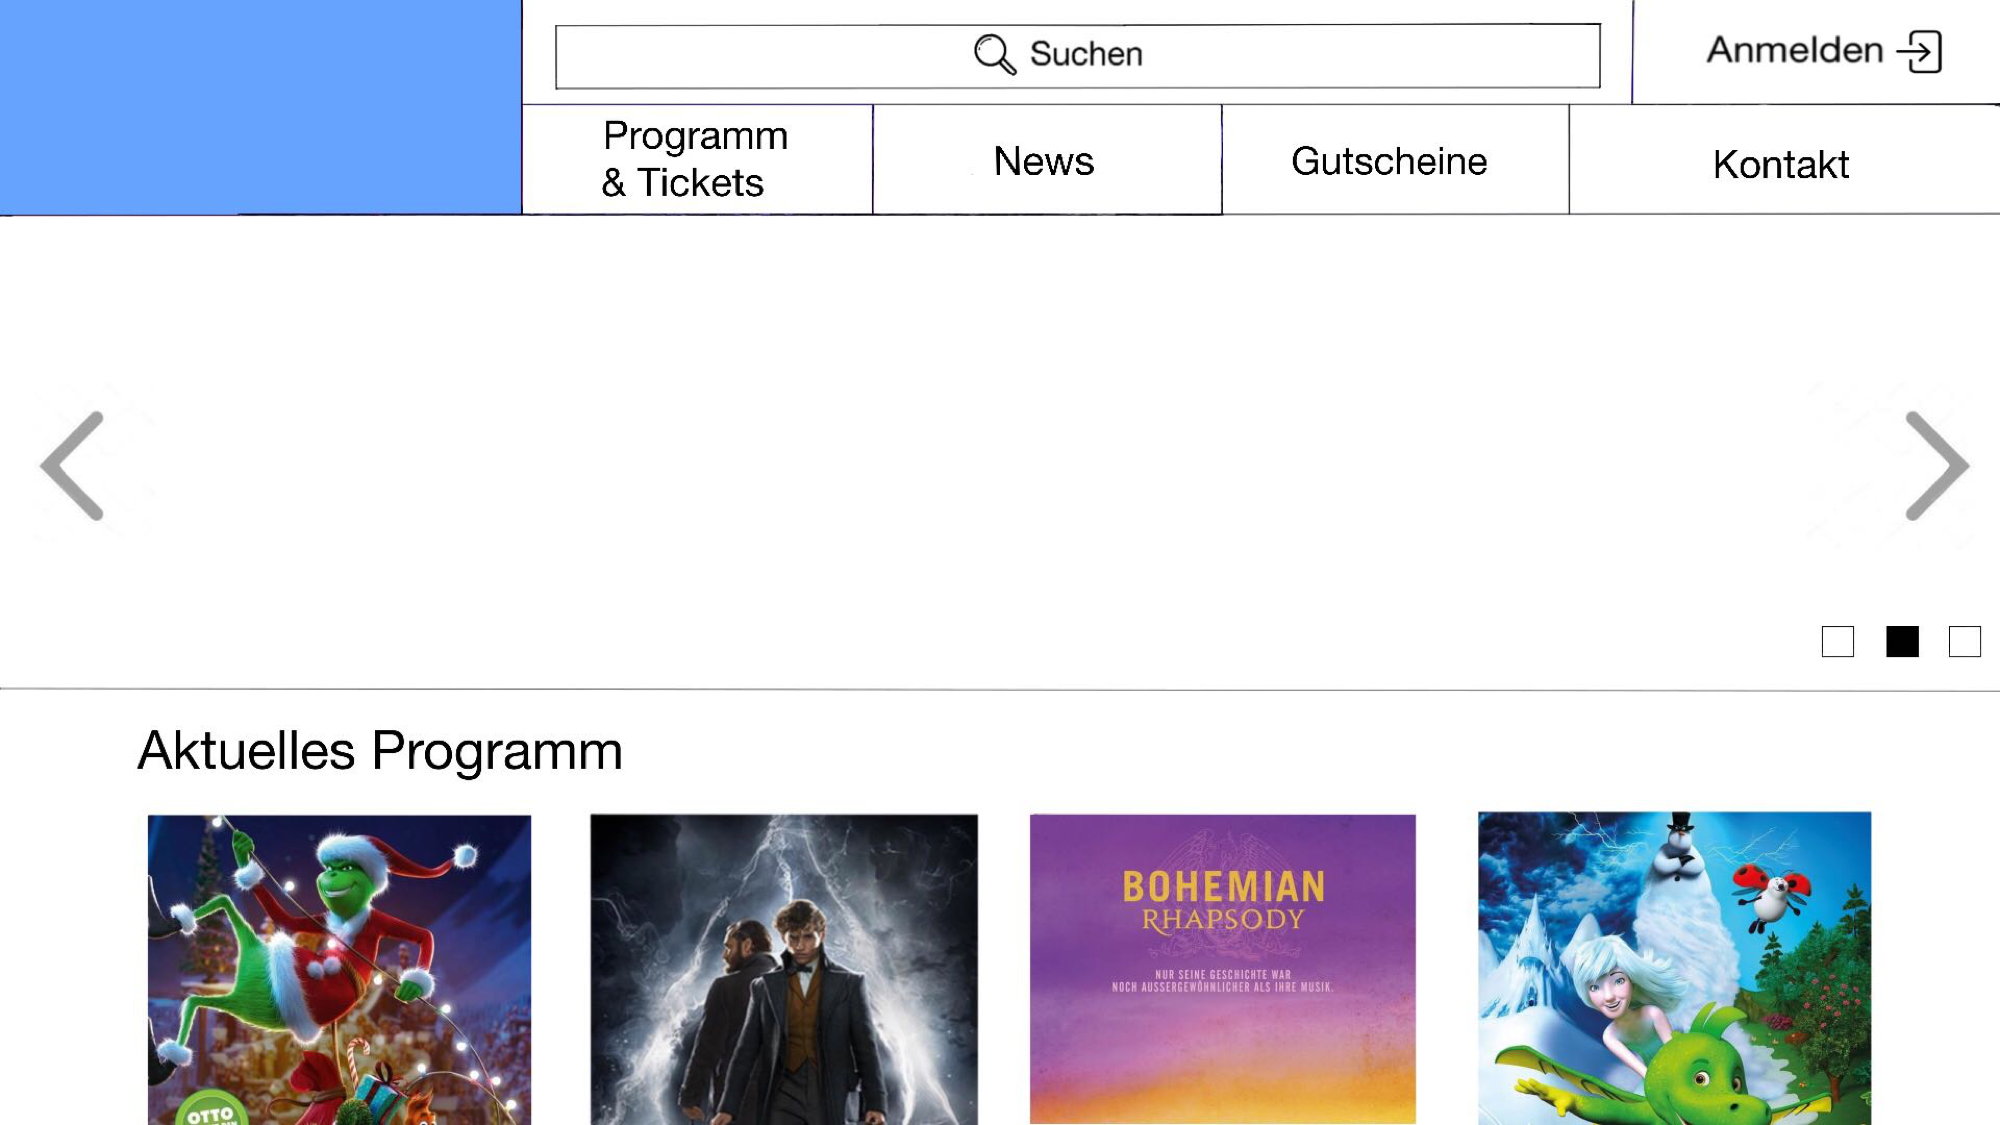
\includegraphics[width=10.8cm]{img/mockUp1.png}
			\captionsetup{format=hang}
			\caption[Mockup Startseite]{\label{fig:mockUpStartseite} Mockup Startseite }
		\end{figure}
		
		Die Navigationsleiste unterscheidet sich zwischen den verschiedenen Seiten nicht. Die blaue Box in der linken, oberen Ecke ist als Platzhalter für das \ac{ICS}-Logo gedacht. Die Navigationsleiste teilt sich in zwei Spalten auf und die einzelnen Sektionen sind eindeutig durch Linien voneinander getrennt. Die Startseite selbst besteht aus einen Slider, welcher möglicherweise aktuelle Filme oder Angebote beinhalten könnte, und dem aktuellen Programm. Dieses wird über die entsprechenden Filmplakate dargestellt, welche einen Link zu fortführenden Informationen implementieren sollen.
		
		\begin{figure}[H]
			\centering 
			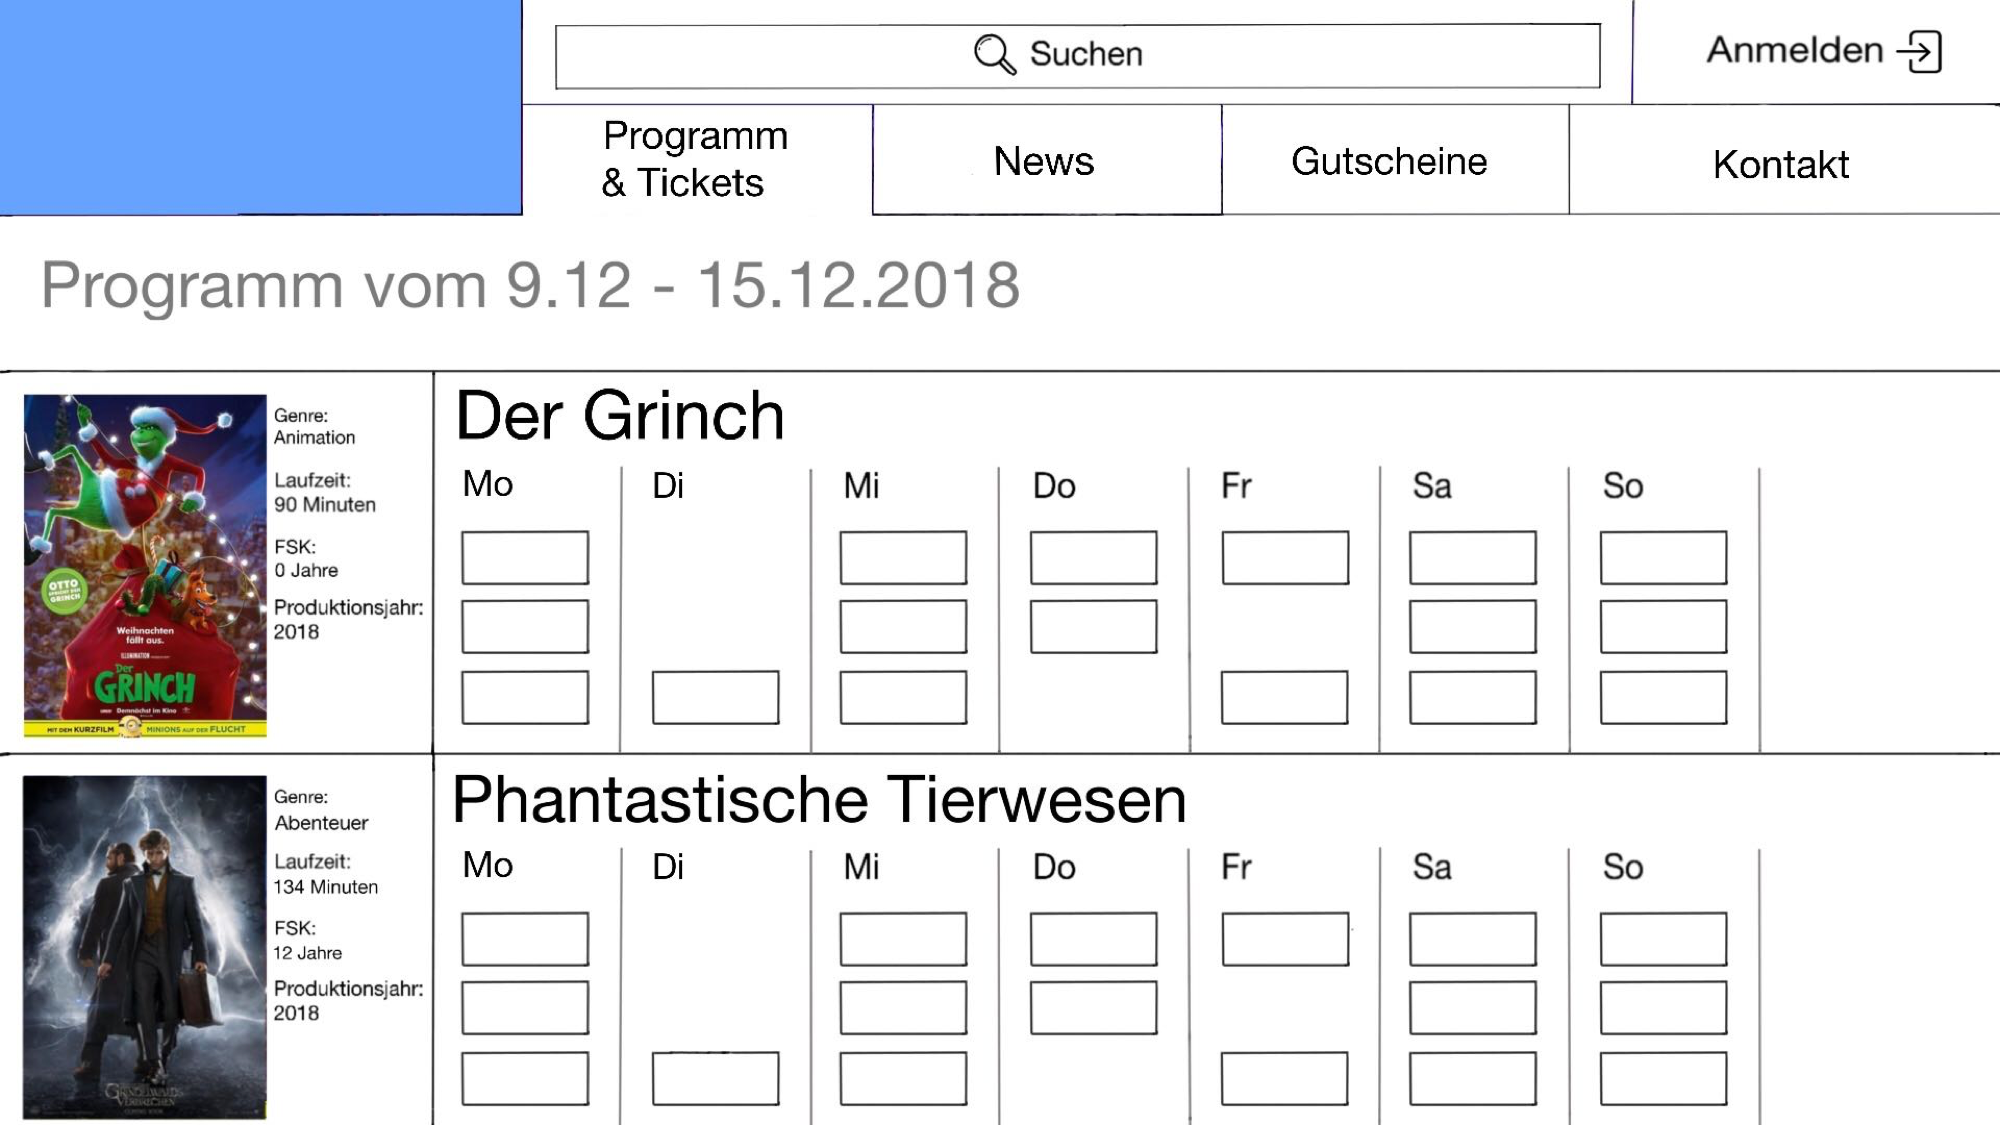
\includegraphics[width=12cm]{img/mockUp2.png}
			\captionsetup{format=hang}
			\caption[Mockup Programm]{\label{fig:mockUpProgramm} Mockup Programm }
		\end{figure}
		
		Die nächste Ansicht zeigt das Programm, also die Filme mit ihren Vorstellungen. Die Filme werden tabellarisch untereinander in Spalten aufgereiht. In jeder Spalte werden auf der linken Seite noch einmal wesentliche Informationen bereitgestellt, während auf der Rechten der Kalenderausschnitt für die jeweilige Woche zu sehen ist. Die Laufzeiten der Filme werden im Mockup als Kästchen symbolisiert, welche später durch entsprechende Uhrzeiten zu ersetzen sind. Diese Kästchen sollen durch einen klick zur nächsten Seite führen: der Detailansicht einer Vorstellung mit Sitzplan.
		
		In Abbildung \ref{fig:mockUpSitzplan} sind noch einmal die Eckdaten der ausgewählten Vorstellung zu sehen. Darunter soll der Nutzer über zwei Eingabefelder die Anzahl, als auch den Typ der gewünschten Plätze auswählen können. Mithilfe des Sitzplans kann nun eine genauere Auswahl der Sitze erfolgen. Die Quadrate, welche die Sitze darstellen sollen, nehmen hierzu passende Farben an und können durch Klicken ausgewählt werden.
		
		\begin{figure}[H]
			\centering 
			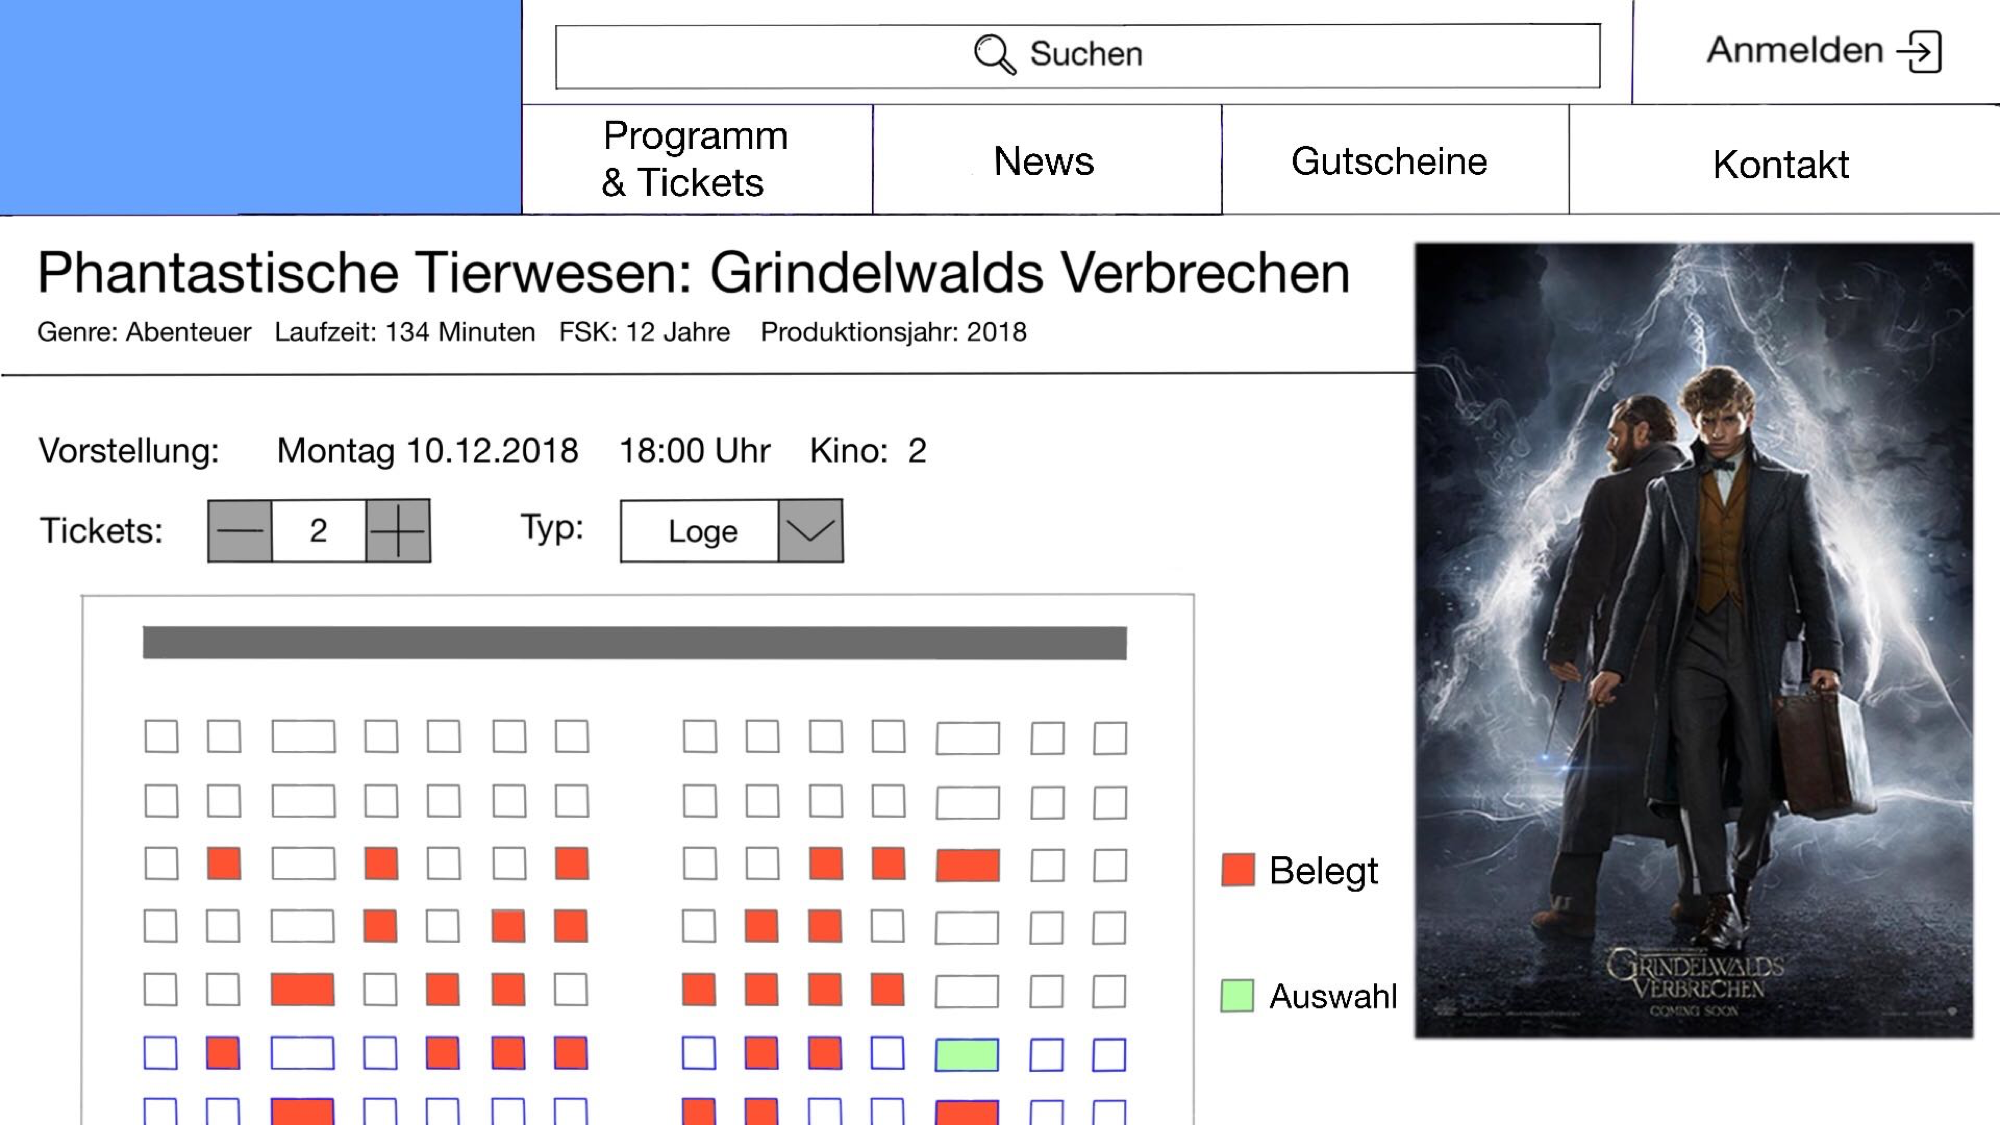
\includegraphics[width=12cm]{img/mockUp3.png}
			\captionsetup{format=hang}
			\caption[Mockup Sitzplan]{\label{fig:mockUpSitzplan} Mockup Sitzplan }
		\end{figure}
		
		
	
	\section[Technischer Entwurf]{Technischer Entwurf{\hfill \normalsize Felix Waage}} 	

		Das \ac{ICS} ist ein komplexes Softwaresystem, welches aus verschiedenen Komponenten, Services und Schichten besteht. Aus diesem Grund war es bereits von Beginn an wichtig, einen genauen Entwurf der späteren Softwarearchitektur zu entwickeln. Diese Vorgehensweise soll vor allem ein möglichst skalierbares, effizientes und anpassungsfähiges Softwaresystem hervorbringen. Des Weiteren wird durch eine gute Dokumentation das System wartungsfreundlicher, da Zusammenhänge schneller erkannt werden können und somit Probleme leichter aufzufinden sind. Auch die Zusammenarbeit der Teammitglieder profitiert von einem ausführlichen technischen Entwurf.
		
			Im weiteren Verlauf dieses Kapitels werden die verschiedenen Schichten erläutert und deren Kommunikation untereinander beschrieben. Darüber hinaus sollen die beteiligten Objekttypen ermittelt und in ein Entitiy-Relationship-Diagramm überführt werden. Das ER-Diagramm dient anschließend als Grundlage für die Entwicklung eines Klassenmodels für das Backend und der Implementierung einer Datenbank für das ICS. 
			
			\subsection{Entwurfsprinzipien}
			Das Ziel der technischen Entwurfsphase ist die Hervorbringung einer skalierbaren, effizienten und anpassungsfähigen Softwarearchitektur. Aus diesem Grund wurden im Vorhinein einige Prinzipien festgelegt, welche bei der Erstellung des technischen Entwurfs beachtet werden sollen, um dieses Ziel zu erreichen.
			%Beim Entwurf eines Softwaresystem ist es besonders wichtig konsistent und gründlich zu arbeiten. Die  Dies ist bedingt durch die Tatsache, dass immer mehrere Personen am \ac{ICS} arbeiten und den Entwurf verstehen müssen.  Aus diesem Grund wurden vor Beginn der Entwicklung des Entwurfs einige Prinzipien festgelegt. Alle Prinzipien, welche folgend aufgelistet und erläutert werden, sollen unter anderem die Übersichtlichkeit, die Wartbarkeit und die Wiederverwendbarkeit des gesamten Projekts oder von Teilen davon ermöglichen.
			\begin{itemize}
				\item \textbf{Das Prinzip einer einzigen Verantwortung} -- Um die Komplexität und Organisation des Softwareprojekts beherrschen zu können, wird das Projekt in verschiedene Module aufgeteilt. Dabei könne einzelene Module wieder aus anderen Modulen zusammen gesetzt sein. Es gilt so Komplexitäten aufzulösen. Jedes Modul übernimmt dabei genau eine Verantwortung und jede Verantwortung wird von genau einem Modul übernommen. Verantwortung ist in diesem Fall die Verpflichtung, eine Anforderung umzusetzen. \autocite[Vgl.][]{Lahres.2015}
				
				\item \textbf{Trennung der Anliegen} -- Jedes Anliegen in einer Anwendung soll durch ein eigenes Modul realisiert werden. Ein mögliches Anliegen wäre zum Beispiel die Transaktionssicherheit, welche unter anderem bei der Reservierung benötigt wird, jedoch auch bei weiteren Anforderung wiederverwendet werden soll.\autocite[Vgl.][]{Lahres.2015} 
				
				\item \textbf{Wiederholungen vermeiden} -- Wenn gleiche Funktionalitäten in einem Softwaresystem mehrfach verwendet werden, sollten diese in ein Modul ausgelagert werden, um mögliche Redundanzen zu vermeiden. Dies könnte vor allem dann zum Problem führen, wenn im Code Fehler entdeckt wurden und dieser Fehler so an mehreren Stellen im Quelltext behoben werden muss. Dies stellt eine große Fehlerquelle dar und sollte somit vermieden werden.\autocite[Vgl.][]{Lahres.2015}
				 
				\item \textbf{Trennung der Schnittstelle von der Implementierung} -- Jedes Modul sollte nur von einer klar definierten Schnittstelle eines anderen Moduls abhängig sein. Dabei spielt die Implementierung der einzelnen Funktionalitäten keine Rolle. Der Quelltext der einzelnen Funktionalitäten soll demnach ausgetauscht werden können, ohne Änderungen an den Schnittstellenaufrufen vornehmen zu müssen. Dies macht das Softwaresystem verständlicher und einfacher zu warten.\autocite[Vgl.][]{Lahres.2015} 
				
				\item \textbf{Testbarkeit} -- Um direkt während der Entwicklung auf Fehler reagieren zu können, ist es wichtig, darauf zu achten, dass sich die einzelnen Module und Softwarekomponenten einzeln testen lassen. So werden neben der eigentlichen Funktionalität auch Unit-Test implementiert. Dies soll möglichst parallel zur Entwicklung der Funktionalität geschehen und muss beim Erstellen des Entwurfs beachtet werden.\autocite[Vgl.][]{Lahres.2015} 
			\end{itemize} 
		
		Wie in vermutlich jedem großen Softwareprojekt kann es zu Sonderfällen kommen, wodurch nicht immer alle Prinzipien genau angewendet wurden. 
		
		\subsection{Schichtenmodell ICS}\label{schichtenmodell}
		
		
		\begin{figure}[H]
			\centering 
			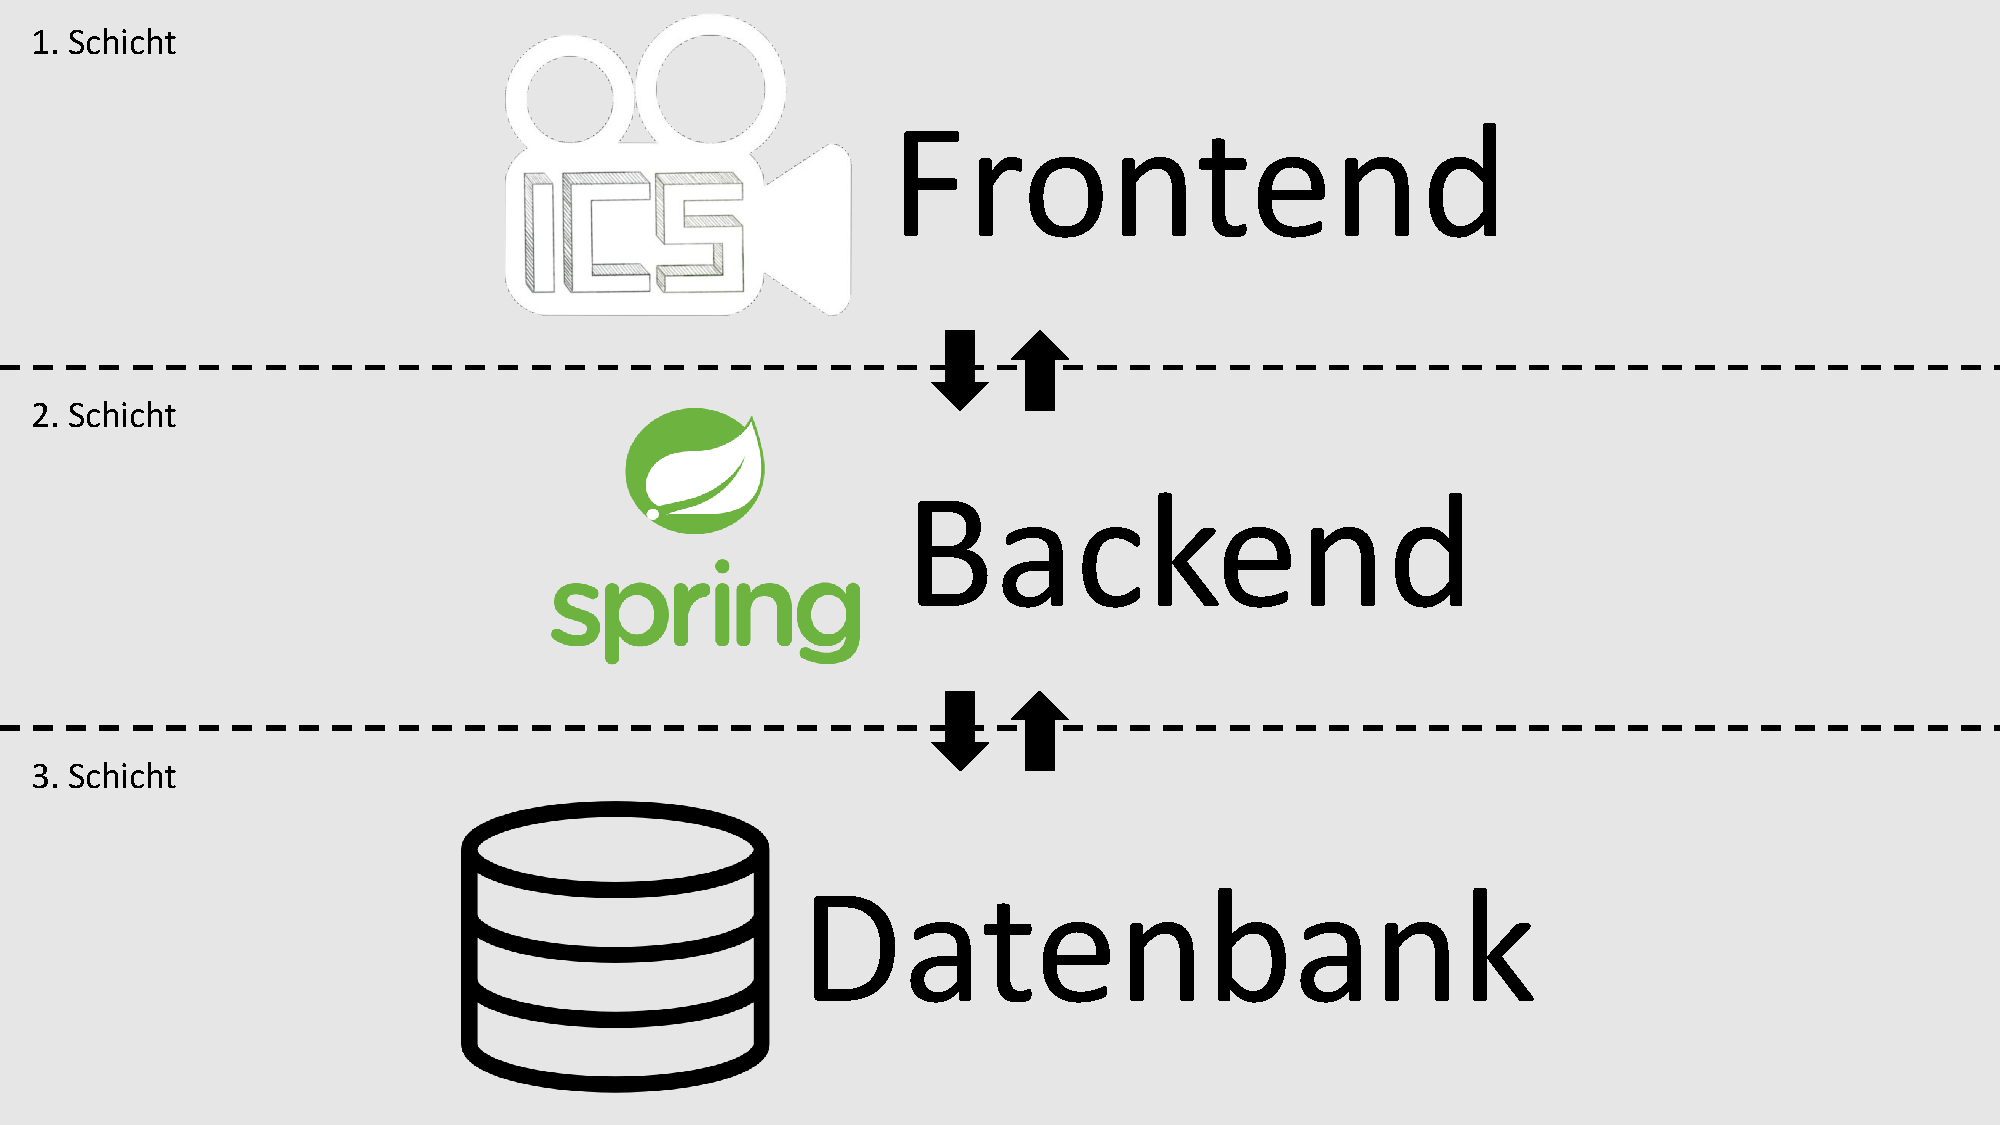
\includegraphics[width=12cm]{img/Schichtenmodell_ICS.pdf}
			\captionsetup{format=hang}
			\caption[Schichtenmodell des ICS]{\label{fig:Schichtenmodell} Schichtenmodell des \ac{ICS} }
		\end{figure}
		
		Die Entwicklung des technischen Entwurfs für das \ac{ICS} wurde damit begonnen, die notwendigen Schichten zu identifizieren und in Relation zueinander zu setzen. Es wurde beschlossen, das Softwaresystem in drei Schichten aufzutrennen. 
		
		Die oberste Schicht ist das \glqq \textbf{Frontend}\grqq{}, welches die grafische Schnittstelle zum Benutzer darstellt. Über das Frontend kann der Benutzer zum Beispiel Filme suchen, Informationen zu Filmen einsehen und Tickets für eine Vorstellung reservieren. Diese Informationen erhält das Frontend durch HTTP-Requests vom Backend.
		
		Im \glqq \textbf{Backend}\grqq{} ist die Fachlogik des Softwaresystem abgebildet, welche zum Beispiel zur Überprüfung der Korrektheit einer Reservierung benötigt wird. Darüber hinaus werden vom Backend die benötigten Rest-Schnittstellen bereitgestellt und die Verbindung zur Datenbank organisiert. 
		
		Die \textbf{Dankbank} dient der Speicherung sämtlicher Daten und Informationen. Sie ist direkt mit dem Backend verbunden und nimmt Anfragen über SQL entgegen. 
		
		Für die Trennung des Softwaresystems in drei Schichten gibt es verschiede Gründe. Zum einen werden für die Implementierung des Frontends andere Technologien verwendet als für das Backend oder die Datenbank. Darüber hinaus verlangen die Anforderungen an das \ac{ICS} eine zentrale Datenhaltung, was sich am besten durch unterschiedliche Schichten realisieren lässt. Darüber hinaus ist durch die Trennung der Schichten eine einfache Skalierung möglich, falls zum Beispiel mehrere Kinos dieses System parallel nutzen möchten.
		\subsection{Entity-Relationship-Modell}\label{chapter:er-diagramm}
		Resultierend aus den Anforderung an das \ac{ICS} gilt es, ein Modell zu entwerfen, welches möglichst genau die spätere Fachlogik repräsentieren kann. Dazu bietet sich für den Anfang das \glqq Entity-Relationship-Modell\grqq{} an.
			
		Das \textit{\glqq Entity-Relationship-Modell\grqq{}} ist ein Datenmodell, welches zur Modellierung von logischen Datenbeziehungen verwendet wird. Der Vorteil in der ER-Modellierung liegt in der einfachen Übertragbarkeit in ein logisches relationales Datenbankmodell, dem \textit{Relationenmodell von Codd}. Ein ER-Diagramm nach der Chen-Notation besteht aus Folgenden Bestandteilen:\autocite[Vgl.][]{Stobitzer.0130201914:40Uhr}
			\begin{itemize}
				\item \textbf{Entität/Entität-Typ} -- Unter einer Entität versteht man ein Objekt der realen Welt (wie z.B.: Avatar, VW Golf, Peter). Gleichartige Entitäten lassen sich anschließend zu einem Entitätstypen zusammenfassen (z.B.: Filme, Autos, Personen).\autocite[Vgl.][]{Stobitzer.0130201914:40Uhr} 
				\item \textbf{Relation} -- Durch die Relation wird die Beziehung zwischen zwei Entitäten beschrieben. So existiert zum Beispiel eine Beziehung zwischen dem Ticket und einer Person. Darüber hinaus ist die Beziehung zwischen zwei oder mehreren Entitäten durch die Kardinalität näher bestimmt. So kann eine Person mehrere Tickets gekauft haben, wobei ein Ticket nur zu einer Person gehört.\autocite[Vgl.][]{Stobitzer.0130201914:40Uhr}
				\item \textbf{Attribut} -- Attribute beschreiben Entitäten näher und enthalten Informationen wie: Name, Alter, Preis.
			\end{itemize}
		
		Die zuvor erwähnte Chen-Notation wird grafisch folgendermaßen grafisch dargestellt (siehe Abbildung \ref{fig:chennotation}).
					\begin{figure}[H]
						\centering 
						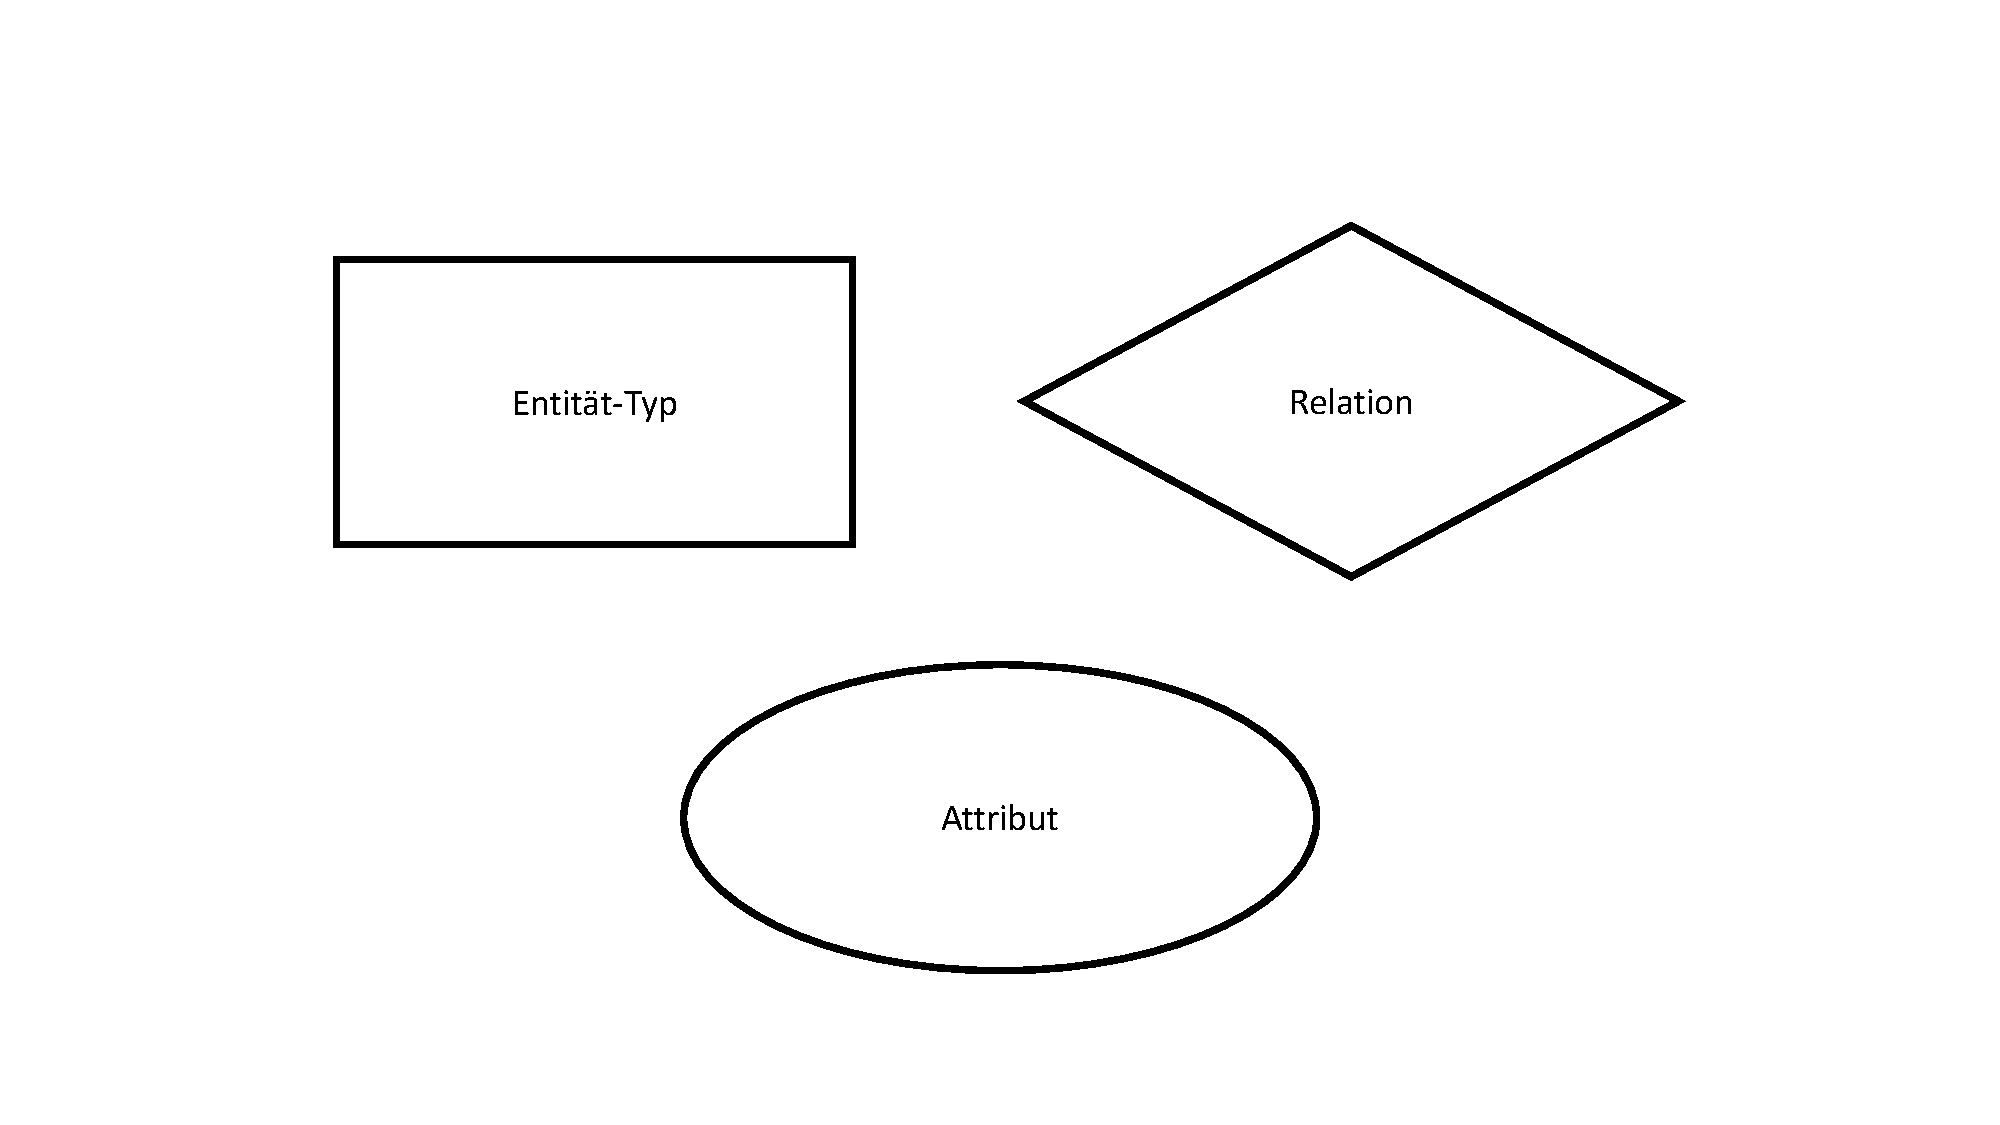
\includegraphics[scale=0.3]{img/ChenNotationERDiagramm.pdf}
						\captionsetup{format=hang}
						\caption[ER-Diagramm Chen-Notation]{\label{fig:chennotation} ER-Diagramm nach der Chen-Notation }
					\end{figure}
		
		Das ER-Diagramm wird auf Grundlage der Ergebnisse der Analysephase erstellt. Dazu werden zu Beginn die beteiligten Entitäten ermitteln. Dies kann besonders gut an der Reservierung eines Tickets erläutert werden. So sind am Reservierungsprozess die Entitäten \textit{Reservierung, Ticket und Benutzer} beteiligt. Im nächsten Schritt werden die Relationen zwischen den Entitäten aufgestellt. Dies kann verbal wie folgt beschrieben werden: Eine Reservierung umfasst immer mindestens ein Ticket. Eine Reservierung wird durch genau einen Benutzer vorgenommen. Aus dieser verbalen Beschreibung der Relationen lassen sich auch die Kardinalitäten bestimmen:
		\begin{itemize}
			\item \textbf{Reservierung \textit{umfasst} Tickets} -- Hier handelt es sich um eine 1:n (n > 0) Beziehung, denn eine Reservierung kann ein oder mehrere Tickets \textit{umfassen}, wobei ein Ticket immer nur zu einer Reservierung gehören kann.
			
			\item  \textbf{Benutzer \textit{macht} Reservierung} -- Eine Reservierung wird immer durch genau einen Benutzer vorgenommen, jedoch kann ein Benutzer mehrere Tickets Reservieren, muss es jedoch nicht, weshalb es sich hier auch um eine 1:n Beziehung handelt, wobei in diesem Fall n auch den Wert 0 annehmen kann. 
		\end{itemize}
		Im letzten Schritt gilt es, die Attribute der einzelnen Entitäten zu ermitteln und in das ER-Diagramm einzutragen. So hat ein Benutzer eine Email-Adresse (\texttt{email}), einen Namen (\texttt{name}) und eine Benutzernummer (\texttt{benutzer\_nr}). Eine Reservierung besitzt eine Reservierungsnummer (\texttt{res\_nr}), ein Datum (\texttt{datum}) und eine Benutzernummer (\texttt{benutzer\_nr}). Und jedes Ticket eine Reservierungsnummer (\texttt{res\_nr}) und eine Ticketnummer (\texttt{ticket\_nr}). Ein Ticket beinhaltet natürlich noch Informationen zur Vorstellung, dem Sitz und dem Preis, jedoch sollen diese zur Vereinfachnung nicht betrachtet werden. Nachfolgend ist das eben erläuterte ER-Diagramm abgebildet (Abbildung \ref{fig:erdiagramm_reservation}).
		
		\begin{figure}[H]
			\centering 
			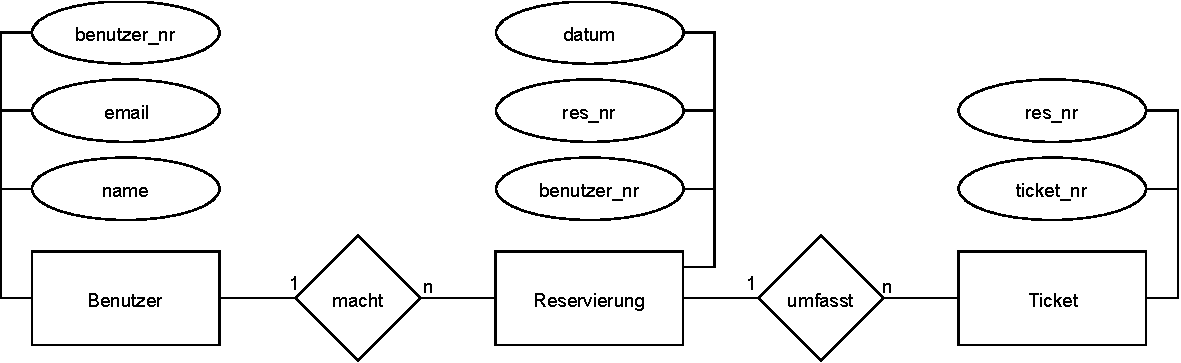
\includegraphics[width=13cm]{img/erdiagramm_reservation.pdf}
			\captionsetup{format=hang}
			\caption[ER-Datenmodell Reservierungsprozess]{\label{fig:erdiagramm_reservation} Entity-Relationship-Diagramm für den Reservierungsprozess}
		\end{figure}
		
		Um die gesamte Funktionalität abbilden zu können, welche in der Analysephase ermittelt wurde, sind weitere Entitäten notwendig. So gehört, wie bereits erwähnt, zu einem Ticket auch eine \texttt{Vorstellung} und eine Vorstellung kann mit	 mehreren Tickets besucht werden. Des Weiteren wird dem Ticket auch ein \texttt{Sitz} zugeordnet und dieser Sitzt befindet sich in einem \texttt{Saal} und ist durch eine \texttt{Sitzkategorie} näher definiert. Einer Vorstellung ist immer genau ein \texttt{Film} zugeordnet, jedoch kann ein Film in mehreren Vorstellungen laufen. Um den Film besser einordnen zu können, steht dieser in Beziehung mit dem \texttt{Genre}. Einem Film kann dabei genau ein Genre zugewiesen werden, wobei mehrere Filme das gleiche Genre besitzen können. Die Preise für ein Ticket ergeben sich aus der \texttt{Sitz-} und \texttt{Vorstellungskategorie}, indem diese jeweils in einer Beziehung zur \texttt{Preiskategorie} stehen. 
		Unter Berücksichtigung der Entitäten und wie diese in Beziehungen zueinander stehen ergibt sich das ER-Diagramm für das \ac{ICS} (Abbildung  \ref{fig:erModell}).
		
		Mit Hilfe des Entity-Relationship-Modell kann nun die Datenbank angelegt werden. Dazu sind bestimmte Regeln und Vorgehensweisen anzuwenden, um die benötigten Tabellen und Spalten aus dem ER-Modell zu extrahieren:
				
		Die Tabellen der Datenbank entsprechen den Entitäten im ER-Modell. Die Attribute werden als Spalten überwiegend unverändert übernommen. Als Schlüssel bietet es sich an, ein zusätzliches Schlüsselattribut zu verwenden, das eine fortlaufende Nummer oder eine \ac{UUID}. Um die Beziehungen zwischen den Attributen richtig abbilden zu können, müssen die Kardinalitäten beachtet werden. 
				\begin{itemize}
					\item 1:1 Beziehung -- Bei dieser Form der Kardinalität enthält eine der beiden Tabellen den Primärschlüssel der anderen Tabelle in Form eines Fremdschlüssels.
					\item 1:n Beziehung -- Liegt diese Form der Kardinalität vor, wird der Primärschlüssel der Entität, die nur einfach in der Beziehung beteiligt ist, als Fremdschlüssel auf der n-Seite hinzugefügt. 
					\item n:m Beziehung -- Sind beide Entitäten in der Beziehung mehrfach beteiligt, gilt es, eine zusätzliche Tabelle anzulegen. Diese enthält die Primärschlüssel der beteiligten Entitäten als Fremdschlüssel.
				\end{itemize}
		
					\begin{figure}[H]
						\centering 
						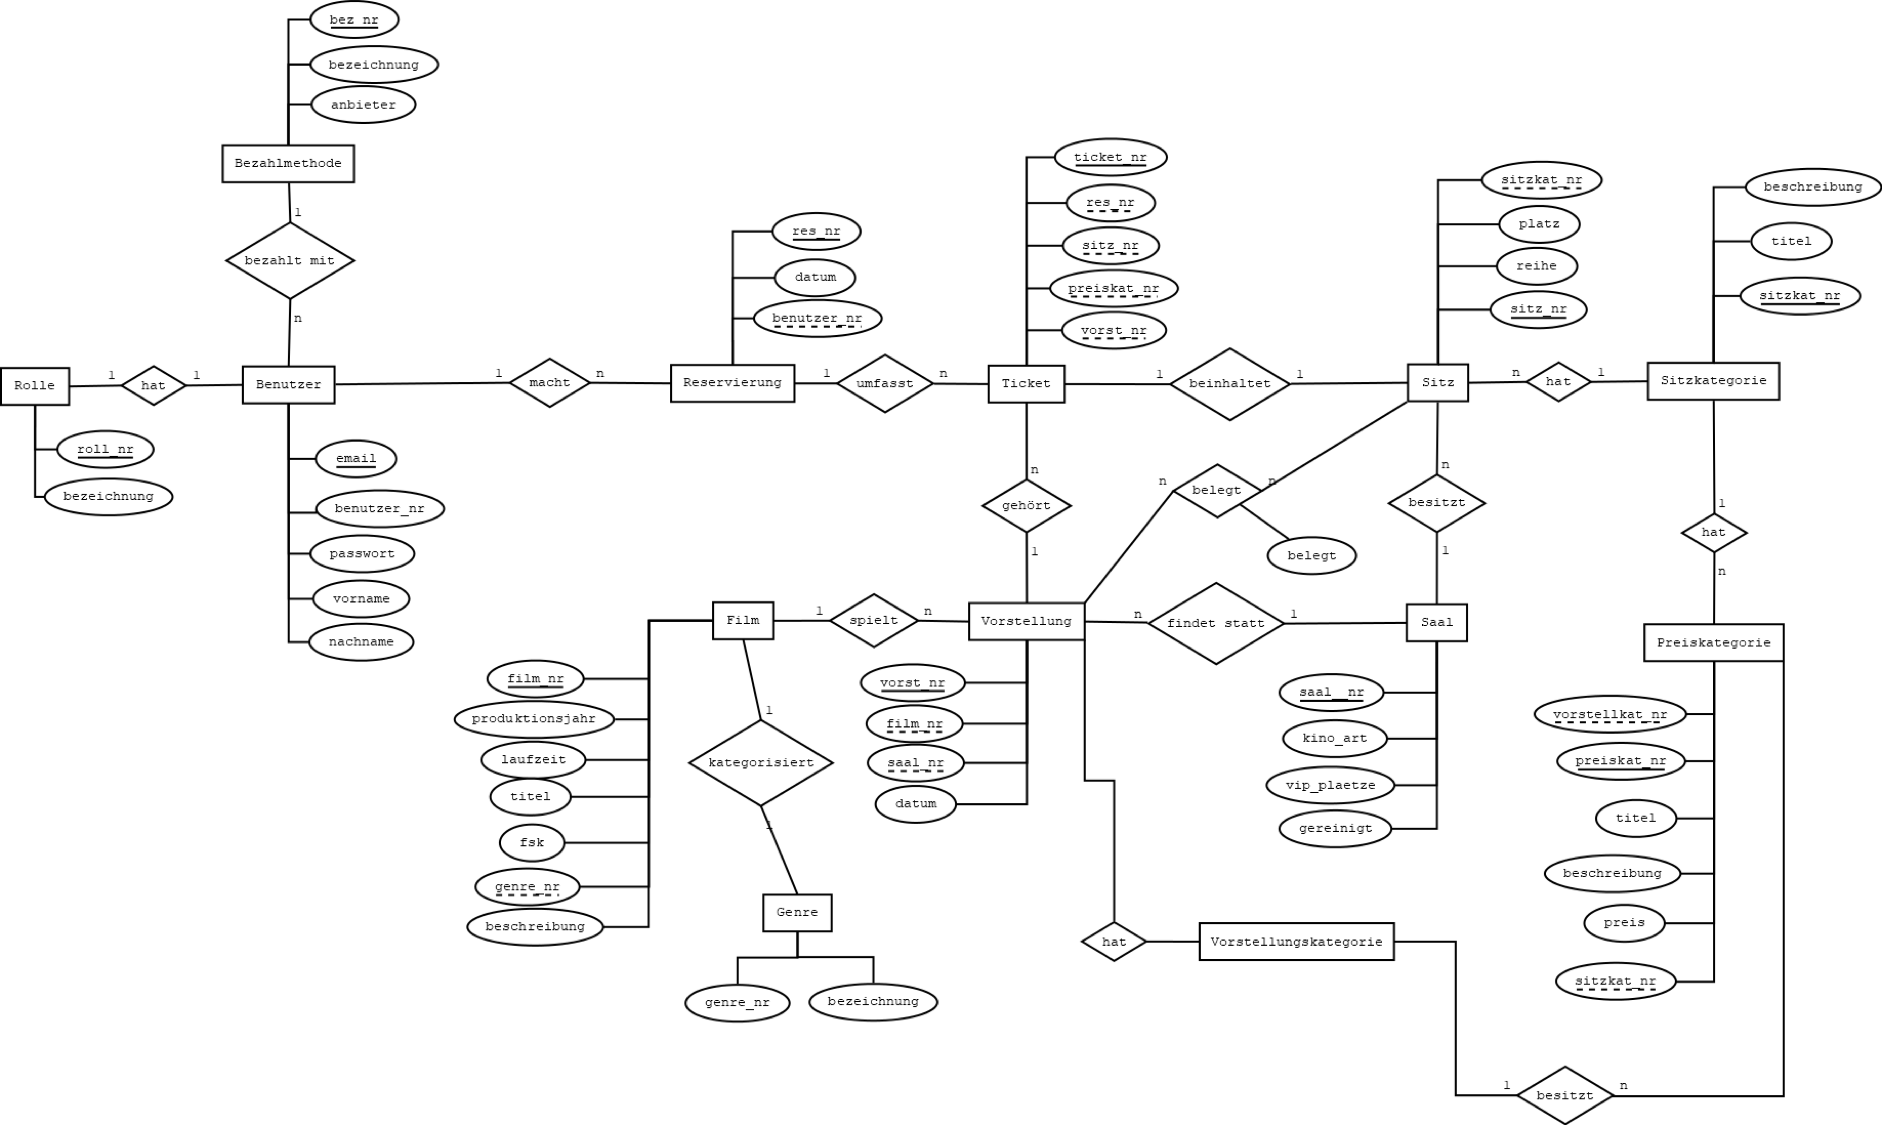
\includegraphics[angle=+90,width=13cm]{img/erModell.png}
						\captionsetup{format=hang}
						\caption[ER-Datenmodell]{\label{fig:erModell} Entity-Relationship-Datenmodell}
					\end{figure}
				
		
		Für das Beispiel des Reservierungsprozesses werden die folgenden Tabellen erstellt: \texttt{Benutzer, Ticket, Reservierung}. Der Benutzer ist an der Beziehung zur Reservierung einfach beteiligt, was dazu führt, dass die Tabelle Reservierung den Primärschlüssel des Benutzers als Fremdschlüssel aufnimmt. Anders verhält es sich bei der Relation zwischen Ticket und Reservierung, denn hier ist die Reservierung einfach beteiligt, wodurch das Ticket den Primärschlüssel als Fremdschlüssel mit speichert. Für dieses Beispiel ergeben sich demnach folgende Datenbanktabellen (Abbildung \ref{fig:database_example}):
		 
		\begin{figure}[H]
			\centering 
			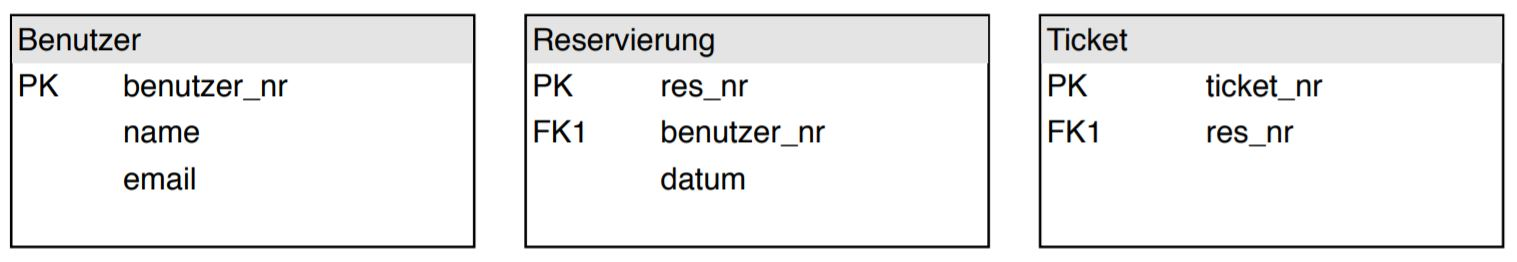
\includegraphics[width=15cm]{img/database_example.JPG}
			\captionsetup{format=hang}
			\caption[Datenbanktabellen Reservierungsprozess]{\label{fig:database_example}Datenbanktabellen für den Reservierungsprozess}
		\end{figure}
		
		\subsection{Klassendiagramm}
		Ein Klassendiagramm dient der strukturierten Darstellung der zu verwendenden Klassen, Schnittstellen sowie deren Beziehungen. Das Klassendiagramm ist die Grundlage für die Implementierung des Backends für das \ac{ICS}, da hier Repräsentanten der Entitäten aus Abschnitt \ref{chapter:er-diagramm} in Form von Java-Objekten benötigt werden, um diese später in der Datenbank speichern zu können. Der Entwurf des Klassendiagramms wurde anhand des zuvor erstellten ER-Diagramms angefertigt. Dabei wurde darauf geachtet, dass die UML-Notation eingehalten wird.
		
		Eine Klasse repräsentiert eine Gruppe von Objekten mit ähnlichen Eigenschaften. Sie besitzt dazu Funktionen und Attribute, welche die Eigenschaften des jeweiligen Objekts definieren. Die einfachste Form einer Klasse ist die anonyme Klasse. Sie wird in UML wie folgt dargestellt (Abbildung \ref{fig:uml_anonym_class}):
		\begin{figure}[H]
			\centering 
			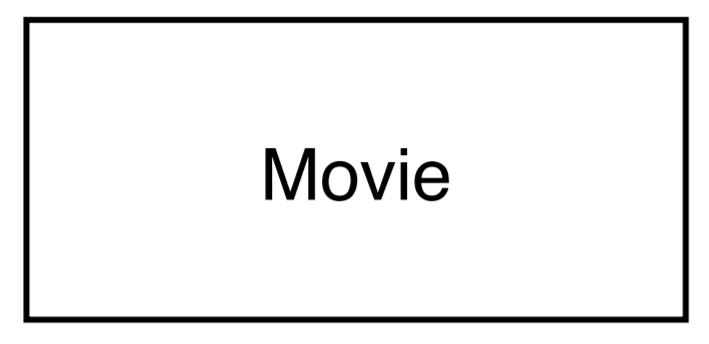
\includegraphics[width=4cm]{img/uml_anonym_class.JPG}
			\captionsetup{format=hang}
			\caption[Anonyme Klasse in UML-Notation]{\label{fig:uml_anonym_class}Anonyme Klasse in UML-Notation}
		\end{figure}
		Diese Darstellung kann durch Attribute und Funktionen erweitert werden, wobei die Sichtbarkeit der Attribute und Funktionen bereits im Klassendiagramm beschrieben werden sollte. In Java sind drei Zugriffsmodifikatoren definiert:
		\begin{itemize}
			\item\textbf{public} -- Es kann von Außen auf das Attribut oder die Funktion direkt zugegriffen werden. Dies kann dazu führen, dass Klassenbestandteile nicht sinngemäß verwendet werden. In UML wird dieser Zugriffsmodifikator durch ein + vor dem Attribut oder der Funktion dargestellt. 
			\item\textbf{private} -- Nur Funktionen innerhalb der Klasse können auf diese Attribute oder Funktionen zugreifen. Die Notation UML beschreibt dies mit einem - vor dem Attribut oder der Funktion.
			\item\textbf{protected} -- Durch den Zugriffmodifikator protected ist es auch Subklassen möglich, auf Attribute und Funktionen zuzugreifen. In der UML-Notation wird dieser Zugriffsmodifikator durch \# repräsentiert.
		\end{itemize}
		Allgemein ist es jedoch üblich, Attribute grundsätzlich als \texttt{private} zu deklarieren und den Zugriff durch sogenannte \textit{Getter- und Setter-Methoden} zu ermöglichen. Dies ermöglicht es, Werte vor dem Speichern auf Korrektheit zu prüfen. Außerdem kann so ein Missbrauch der Klasse für andere Zwecke verhindert werden. Eine Klasse mit all den erwähnten Bestandteilen wird in UML wie folgt dargestellt (Abbildung \ref{fig:KlasseUML}): 
		\begin{figure}[H]
			\centering 
			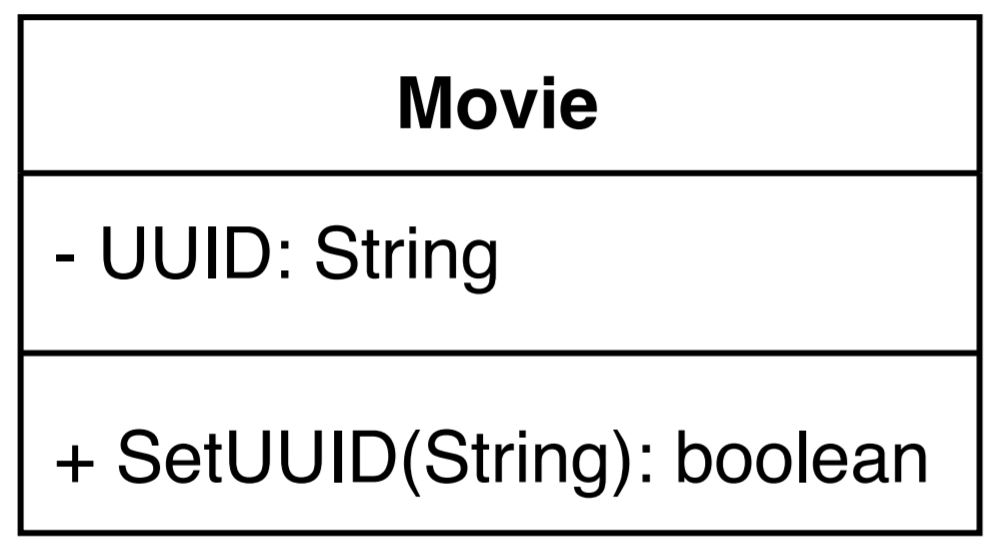
\includegraphics[width=4cm]{img/uml_class.JPG}
			\captionsetup{format=hang}
			\caption[Klasse in UML-Notation]{\label{fig:KlasseUML}Klasse nach der UML-Notation}
		\end{figure}
		Die Relationen zwischen den Klassen werden durch Pfeile und Linien visualisiert, welche wie beim ER-Diagramm an den Enden die Kardinalität der Beziehung angeben. 
		
		\begin{figure}[H]
			\centering 
			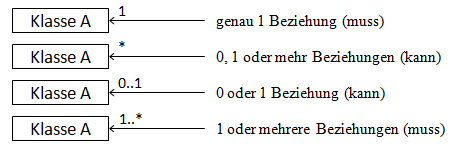
\includegraphics[width=12cm]{img/UmlKardinalitaet.png}
			\captionsetup{format=hang}
			\centering\caption[Kardinalitäten nach UML-Notation]{\label{fig:Kardinalitaeten.UML}Startseite von Kinopolis\footnotemark}
		\end{figure}\footnotetext{Quelle: http://www.info-wsf.de/index.php/Assoziationen\_und\_Kardinalit\%C3\%A4ten}
		
		Neben den Kardinalitäten werden auch Aggregationen und Kompositionen in der UML-Darstellung ermöglicht. Eine \textit{Aggregation} ist eine besondere Form der Beziehung zwischen zwei Klassen. Sie drückt aus, dass eine Klasse Objekte der anderen Klasse als Attribut beinhaltet. Verbal wird dies oft mit \textit{besteht aus, hat, ist Bestandteil von} ausgedrückt. Eine Komposition ist ähnlich zur Aggregation mit dem Unterschied, dass die Existenz der einen Klasse von der Existenz der anderen abhängt. So kann zum Beispiel ein Raum nicht ohne ein Gebäude existieren. In UML wird dies wie folgt dargestellt:
		
		\begin{figure}[H]
			\centering 
			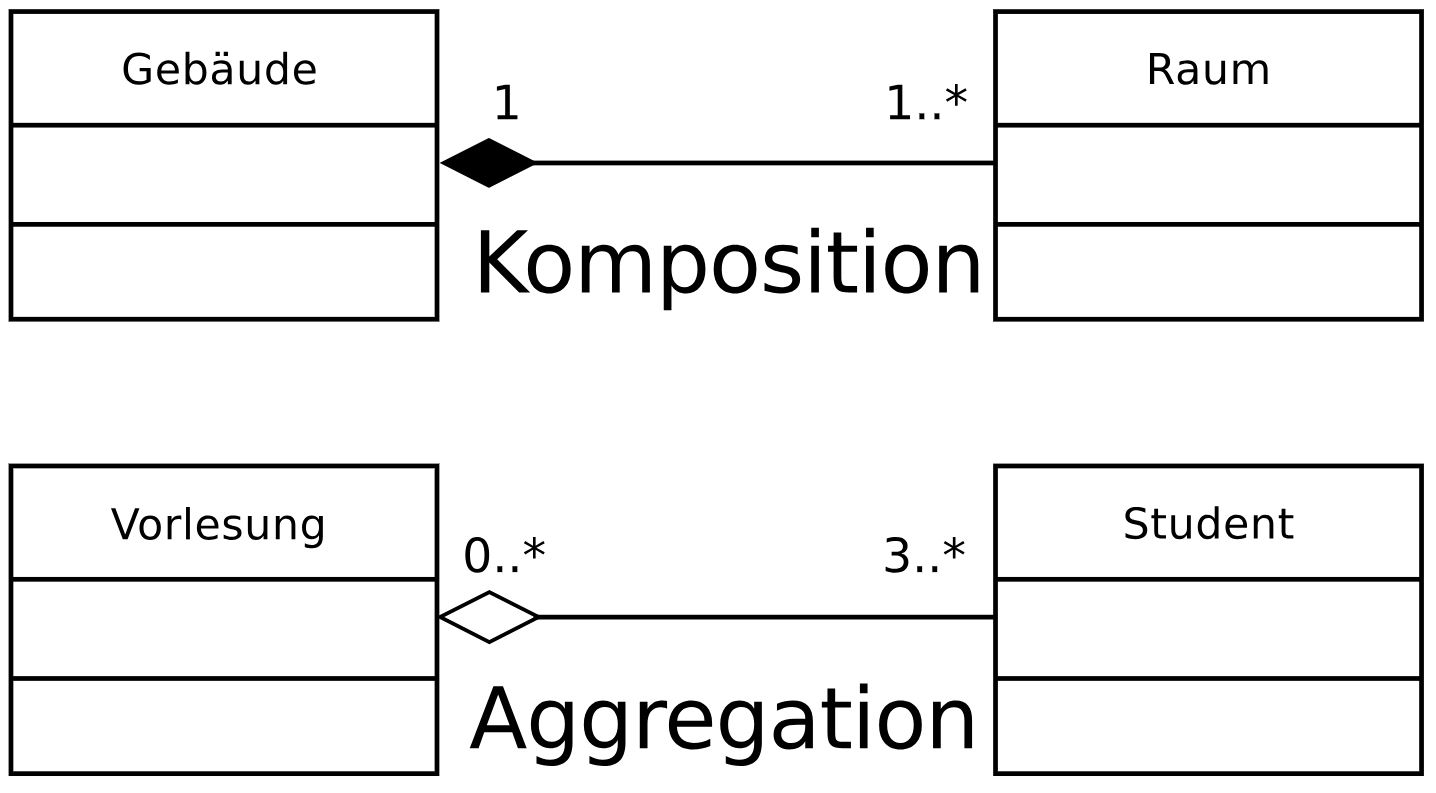
\includegraphics[width=8cm]{img/aggregation_komposition.JPG}
			\captionsetup{format=hang}
			\caption[Aggregation und Komposition]{\label{fig:aggreagtion_komposition}Aggregation und Komposition}
		\end{figure}
		
		Um nun den Reservierungsprozess im Backend abbilden zu können, werden die in Abschnitt \ref{chapter:er-diagramm} ermittelten Entitäten (\texttt{Reservierung, Ticket, Benutzer}) jeweils als eine eigene Klasse implementiert. Da in der Beziehung zwischen Benutzer und Reservierung die Reservierung einfach beteiligt ist, ist der Benutzer Teil von einer Reservierung. Dies wird durch eine Assoziation abgebildet. Ähnlich verhält sich dies in der Beziehung zwischen Ticket und Reservierung. Hier ist die Reservierung einfach beteiligt, weshalb eine Reservierung Teil von einem Ticket ist. Dieser Ausschnitt aus dem Klassendiagramm ist wie folgt grafisch nach UML-Notation abzubilden (Abbildung \ref{fig:reservation_process}):
		
		\begin{figure}[H]
			\centering 
			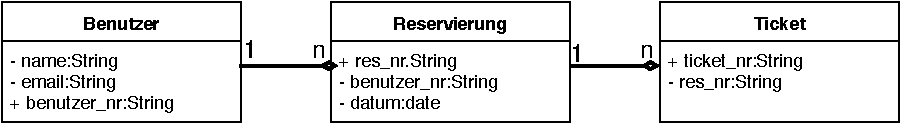
\includegraphics[width=15cm]{img/reservation_process.pdf}
			\captionsetup{format=hang}
			\caption[Klassendiagramm für den Reservierungsprozess]{\label{fig:reservation_process}Klassendiagramm für den Reservierungsprozess}
		\end{figure}
		
		Nach diesem Vorgehen wurde das komplette Klassendiagramm für das \ac{ICS} erstellt, jedoch ist wichtig anzumerken, dass ein erster Entwurf nicht die endgültige Lösung darstellt und während des Entwicklungsprozesses weitere Änderungen im Vergleich zum ER-Diagramm vorgenommen wurden. Aus diesem Grund wird in Abbildung \ref{fig:Klassendiagramm} ein automatisch generiertes Klassendiagramm gezeigt, welches den aktuellsten Stand der Anwendung repräsentiert.
		
		\begin{figure}[H]
			\centering 
			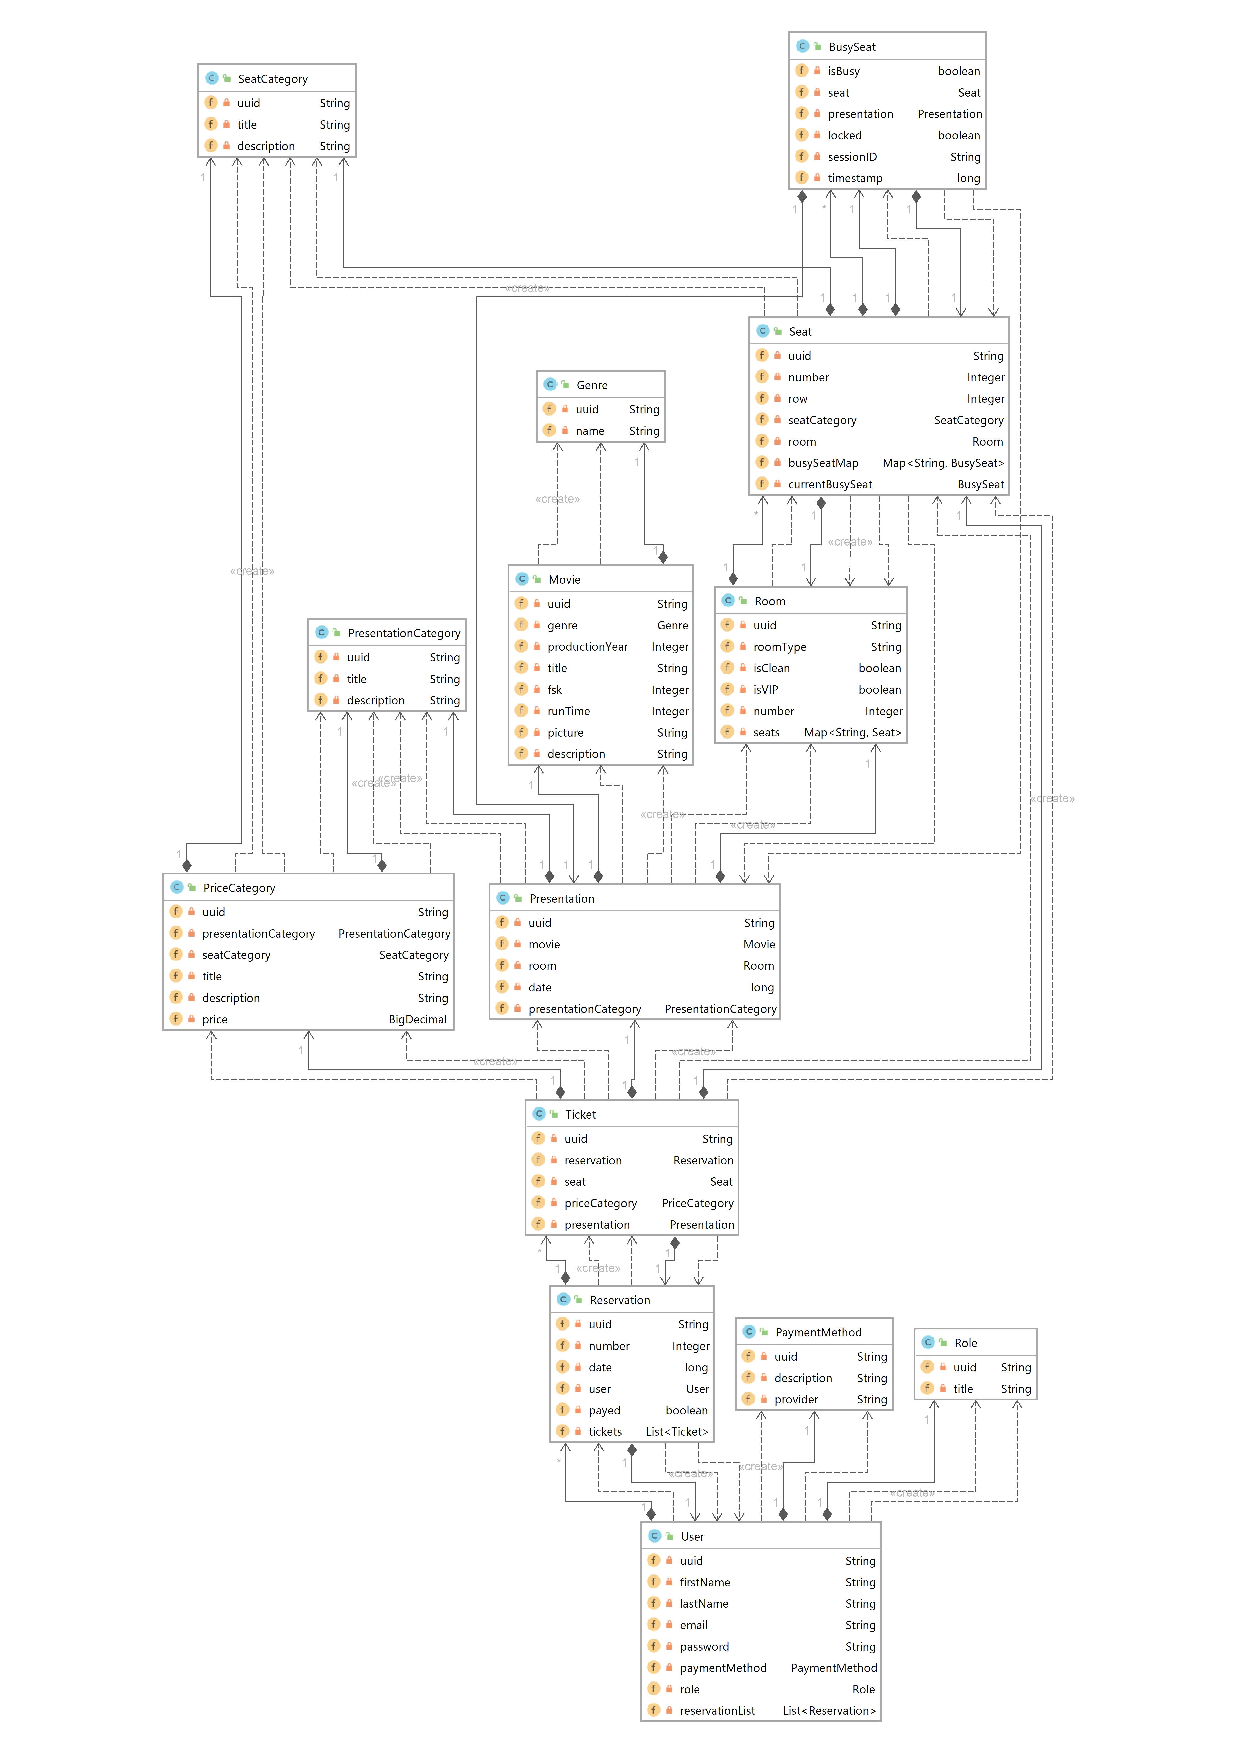
\includegraphics[width=15cm]{img/class_diagramm.pdf}
			\captionsetup{format=hang}
			\caption[Klassendiagramm]{\label{fig:Klassendiagramm}Klassendiagramm}
		\end{figure}
			
		\subsection{Dynamische Modelle}
		Als dynamisches Modell wurde ein Aktivitätsdiagramm gewählt. Dieses veranschaulicht die Abläufe in einem System und beruht auf einem Use-Case des Systems. Ein Aktivitätsdiagramm beinhaltet verschiedene \enquote{Knoten}, die einen elementaren Vorgang im System darstellen. Sie werden auch Aktionen genannt, die zu Aktivitäten zusammengefasst werden können. Um die Knoten zu verbinden und in eine Reihenfolge zu bringen, werden \enquote{Kanten} verwendet. Diese werden mittels Pfeilen dargestellt, wodurch die Reihenfolge vorgegeben wird. 
				
		Beginn und Ende einer Aktivität werden mithilfe eines ausgefüllten Punktes dargestellt, wobei der Endpunkt der Aktivität von einem Kreis umgeben ist. Verzweigungen können in einem Aktivitätsdiagramm mittels \enquote{Rauten} dargestellt werden. Dabei wird textuell hinzugefügt, um welche Entscheidung es sich handelt. 
				
		Abbildung \vref{fig:aktivitätReservierung} veranschaulicht die Aktionen, die ein Benutzer durchläuft, um Karten reservieren zu können. Er startet mit dem Ansehen der Startseite und endet mit einer erfolgreichen Reservierung. Dabei kann der Benutzer zunächst auf der Startseite nach einem passenden Film suchen. Wenn dort kein passender Film vorhanden ist, kann der Nutzer in die Programmübersicht wechseln. Sollte dort ebenfalls kein passender Film vorhanden sein, endet die Aktivität an dieser Stelle. 
								
		Falls jedoch ein passender Film auf Startseite oder Programmübersicht vorhanden ist, besteht die nächste Aktion aus dem Anklicken des Films. Nachfolgend wählt der Benutzer eine Vorstellung und die gewünschten Sitze aus. Die Reservierung wird im Hintergrund ausgeführt, wodurch das Sperren der ausgewählten Sitze vorgenommen wird, falls diese noch nicht gesperrt sind. Für den Fall, dass die Sitze bereits durch einen anderen Nutzer gesperrt sind, wird der Benutzer zur Auswahl von Sitzen zurückgeführt. 
								
		Wenn die Sitze noch frei sind, können diese durch die Eingabe der Benutzerdaten, bei Reservierung als Gast, reserviert werden. Das System prüft die Vollständigkeit der Angaben. Bei Unvollständigkeit wird der Nutzer wieder zurück zu der Auswahl der Sitze geführt. Andernfalls wird die Reservierung bestätigt und der Benutzer kann die Bestätigung einsehen. Damit ist der Reservierungsvorgang abgeschlossen und die Aktivität endet.   
						 
		Informationen zu den Aktionen, die in Frontend und Backend vorgenommen werden, um die Aktion eines Benutzers umzusetzen, können dem Anhang \vref{fig:adResAusführlich} entnommen werden.
				
		\begin{figure}[H]
			\centering 
			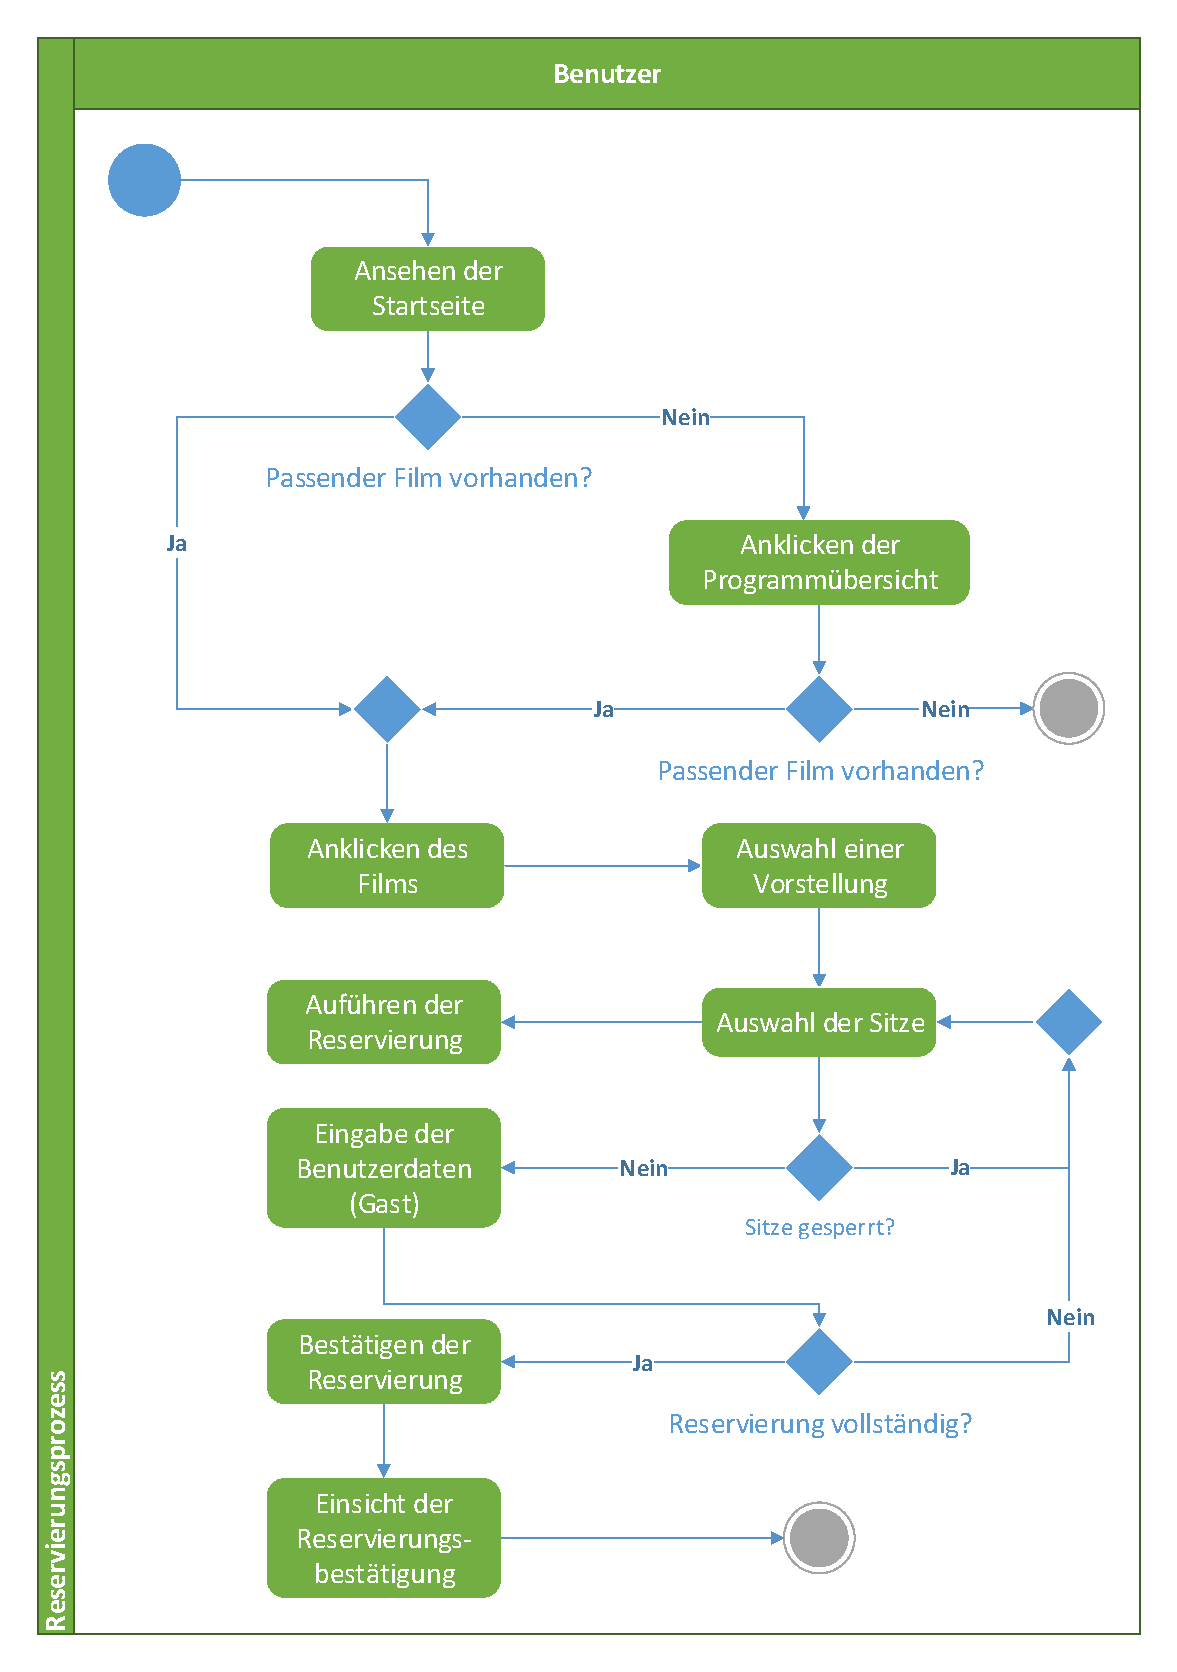
\includegraphics[width=12cm]{img/adReservierung_min.pdf}
			\captionsetup{format=hang}
			\caption[Aktivitätsdiagramm Reservierung]{\label{fig:aktivitätReservierung} Aktivitätsdiagramm Reservierungsvorgang}
		\end{figure}
				
			
% !TEX root =  master.tex
\chapter{Umsetzung} \label{umsetzung}
	\section[Organisation]{Organisation{\hfill \normalsize Sandra Keller}}
	GitHub
	\section[Backend]{Backend{\hfill \normalsize Martin Sandig}}
	
	\subsection{Frameworks}
	
	\subsection{Datenbank}
	
	\subsection{Fachkonzept}
	
	\subsection{Restschnittstellen}
	
	\section[Frontend]{Frontend {\hfill \normalsize Jonas Dutzi, Dennis Köhler}}
	\section[Modultests]{Modultests{\hfill \normalsize Fabio Westphal}}
	Das Testen von Code stellt einen essenziellen Teil der Entwicklung von Software dar. Der ANSI/IEEE Standard 610.12-1990 definiert Tests folgendermaßen:	\enquote {An activity in which a system or component is executed under specified conditions, the results are observed or recorded, and an evaluation is made of some aspect of the system or component.} Man unterscheidet grundsätzlich Whitebox- und Blackbox-Tests. Bei Whitebox-Tests wird die innere Funktionsweise der Software getestet, wohingegen bei Blackbox-Tests kein Wissen über den Quellcode zugrundeliegt und nur der geforderte Funktionsumfang getestet wird.\autocite{franz2007handbuch}[Vgl.][S.28] Im Projekt wurden hauptsächlich Komponententests angewendet, welche zu den Whitebox-Tests zählen. Hierbei werden Klassen und Methoden einzeln parallel zur weiteren Entwicklung getestet. Durch die kleinschrittige Testweise tragen sie auch zur lebenden Dokumentation bei. Wichtig ist dabei, dass jeder Test korrekt,
schnell, abgeschlossen,	isoliert, sprechend benannt, wartbar und einfach durchführbar
ist.
	Es muss der gesamte Code einmal durchlaufen werden, um maximale Korrektheit zu sichern.\autocite{witte2015testmanagement}[Vgl.][S.50] Bei überschauberen Systemen kann man aber auch nur kritische Teile testen. Um die Tests automatisiert auszuführen, werden Test-Frameworks verwendet. In diesem Projekt wird das bekannte Framework JUnit benutzt.
	Bei Datenbankzugriffsklassen ist es vor allem wichtig, die \ac{CRUD}-Operationen zu testen. Diese gelten als die essenziellen Funktionen, wenn es um den Zugriff auf Datenbanken geht. Im Projekt wurde dafür die Klasse \texttt{DaoTestHelper} verwendet, die entsprechende Schnittstellen für die Testklassen zur Verfügung stellt. Im Zuge eines Tests werden zunächst Beispielobjekte erzeugt und persistiert. Anschließend werden die Grundoperationen mithilfe der Helper-Klasse getestet. Am Beispiel der Klasse \texttt{MovieDaoTest} sieht das wie folgt aus:
	\begin{lstlisting}
public class MovieDaoTest {

	private static Movie movie;
	private static Genre genre;
	
	@Autowired
	private GenreDao genreDao;
	
	@Autowired
	private MovieDao movieDao;
	
	@BeforeClass
	public static void setUp() throws Exception {
		movie = new Movie(2015, "TestMovie", "Nice Test Movie", 12, 120);
		genre = new Genre("testGenre");
		movie.setGenre(genre);
	}
	
	@Test
	public void test1Persist() {
		assertFalse(this.movieDao.persist(movie));
		assertTrue(this.genreDao.persist(genre));
		DaoTestHelper.persist(this.movieDao, movie);
	}
	
	@Test
	public void test2Get() {
		DaoTestHelper.get(this.movieDao, movie, movie.getUuid());
	}
	
	@Test
	public void test3GetAll() {
		DaoTestHelper.getAll(this.movieDao, movie);
	}
	
	@Test
	public void test4Update() {
		Movie testMovie = new Movie(movie.getUuid(), 2000,"updatedMovie", movie.getDescription(), movie.getFsk(), movie.getRunTime());
		testMovie.setGenre(movie.getGenre());
		DaoTestHelper.update(this.movieDao, movie.getUuid(), movie, testMovie);
	}
	
	@Test
	public void test5Delete() {
		DaoTestHelper.delete(this.movieDao, movie.getUuid());
	}
}
	\end{lstlisting}
	Beim Ausführen der Tests gibt es in der Entwicklungsumgebung IntelliJ die Möglichkeit, die Abdeckung zu berechnen. Dabei werden zum einen die Zeilen gezählt, die von den Tests betroffen sind und zum anderen die Methoden bzw. Klassen. In Relation zur Gesamtheit der Zeilen - bzw. Methoden oder Klassen - ergibt dies die Testabdeckung als Prozentzahl (siehe Abb. \ref{fig:TestCoverage}).\newline
	\begin{figure} 
		\centering 
		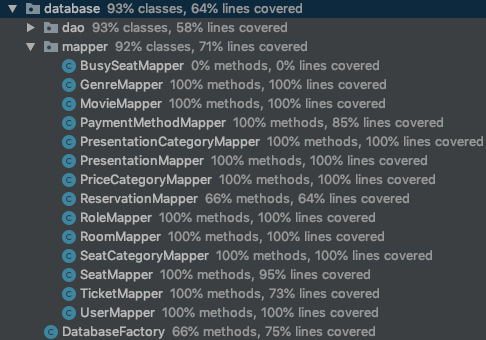
\includegraphics[scale=0.6]{img/testCoverage.png}
		\captionsetup{format=hang}
		\centering\caption[Testabdeckung]{\label{fig:TestCoverage} Übersicht der Testabdeckung}
	\end{figure}
	Die Testabdeckung ist häufig ein faktisches Kriterium für die Qualität des Codes bei Abnahme des Projekts. Beim Erreichen einer bestimmten Prozentzahl fällt allerdings auf, dass diese beim Schreiben der Tests nicht linear steigt. Das liegt daran, dass viele Klassen, die explizit getestet werden, Methoden anderer Klassen wie beispielsweise Superklassen oder Helper-Klassen nutzen. Somit werden diese direkt auch getestet. Andere Klassen wiederum verwenden genau die gleiche Superklasse (oder Helper-Klasse...), die bereits zuvor fremdgetestet wurde. Es sind also weniger Zeilen Code, die für die Testabdeckung zählen, obwohl ähnlich viele Zeilen durchlaufen werden. Daher ist es in der Regel der Fall, dass bei den ersten Tests die Testabdeckung stark wächst, dann jedoch immer langsamer.
	
	\section[Verknüpfung Back- und Frontend]{Verknüpfung Back- und Frontend {\hfill \normalsize tba}}
	REST
	
	\section[Ausblick]{Ausblick {\hfill \normalsize Milena Zahn}}\label{Ausblick}
	%\subsection{Lessons Learned} 
	Die Bereiche, an denen gearbeitet wurde, waren vielfältig. Zuerst waren alle an der Analyse sowie der Erarbeitung des Entwurfs beteiligt. Dann musste sich das Team erarbeiten, wie ein solches Projekt umgesetzt werden kann. Die Programmierung des Backends war für einige der Teammitglieder komplett neu, aber da das Team sehr unterschiedliche Fähigkeiten besitzt, war dies in der geplanten Projektzeit möglich. Auch die Erstellung des Frontends war eine interessante Erfahrung. Die Verbindung von diesem mit dem Backend war für die meisten von uns eine weitere Herausforderung, da in diesem Bereich noch wenige Erfahrungen gemacht wurden. 
	Neben dem technischen Wissen haben die Teammitglieder auch einige weitere Kompetenzen in dem Projekt erworben. Eine davon ist, dass es sehr wichtig ist, andere Projekte, an denen die Teammitglieder außerhalb des Moduls arbeiten müssen, bei dem Projektplans zu berücksichtigen. Obwohl dies sehr schwierig ist, kann dies helfen, den Projektplan genauer und realistischer zu erstellen. Es ist sehr wichtig, für jede Aufgabe genügend Zeit einzuplanen, um unerwartete Herausforderungen zu bewältigen. Die selbständige Erarbeitung von Vorgehensweisen und Lösungskonzepte ist eine weitere in diesem Projekt erworbene Kompetenz.
	Eine weitere Hürde war die Gruppengröße von acht Personen. Es ist schwierig das Potenzial der Gruppe voll ausschöpfen, weil die Arbeit innerhalb der Gruppe gut organisiert werden muss.  Um eine übermäßige Koordination der Mitglieder und lange Kommunikationswege zu vermeiden, haben wir die Gruppe in Untergruppen mit verschiedenen Aufgabenbereichen aufgeteilt. Somit konnte eine schnelle Entscheidungsfindung und kurzfristige Absprachen garantiert werden. Insgesamt wurden in der engen Projektzeit viele unterschiedliche Kompetenzen erworben und vor allem die theoretischen Inhalte der Vorlesung Systemanalyse angewandt.
	
% !TEX root =  master.tex
\chapter{Evaluation}
	Alles subba.
%% !TEX root =  master.tex
\chapter{Ausblick}
	Hätte, hätte, Fahrradkette.

	Fragt man sich immer woran hats gelegen


%	Literaturverzeichnis
\ihead{} % Neue Header-Definition
\printbibliography[title=Literaturverzeichnis]
\cleardoublepage

% Der Anhang beginnt hier - jedes Kapitel wird alphabetisch aufgezählt. (Anhang A, B usw.)
%\appendix
%\ihead{\appendixname~\thechapter} % Neue Header-Definition

% appendix.tex einziehen
%\chapter{Testanhang}

\section{Subtestanhang}

\chapter{Noch ein Testanhang}



% Ehrenwörtliche Erklärung ewerkl.tex einziehen
% !TEX root =  master.tex

\clearpage
\chapter*{Ehrenwörtliche Erklärung}

% Wird die folgende Zeile auskommentiert, erscheint die ehrenwörtliche
% Erklärung im Inhaltsverzeichnis.

 \addcontentsline{toc}{chapter}{Ehrenwörtliche Erklärung}
Wir versicheren hiermit, dass wir die vorliegende Seminararbeit
 mit dem Thema: \textit{\DerTitelDerArbeit} selbstständig verfasst und keine anderen als die angegebenen Quellen und
Hilfsmittel benutzt haben. Wir versicheren zudem,
dass die eingereichte elektronische Fassung mit der gedruckten Fassung übereinstimmt.

\vspace{4cm}
Ort, Datum 

\end{document}
